% =============================================================================
% main.tex  —  IEEE Journal Paper
% Title:  Post-Quantum Readiness of a Lightweight XOR+Hash Mutual
%         Authentication Scheme: An ECC Comparison for Cloud-IoT
% Author: Surya Pratap Singh Raikuni (24BYB1114)
%         Department of B.Tech Cybersecurity, VIT Chennai
% Supervisor: Dr. Karthika V
%
% Compile with pdfLaTeX on Overleaf.
% Switch between journal and conference mode by toggling the two lines below.
% =============================================================================

% =============================================================================
% FORMAT SELECTION: Choose your desired layout mode below (uncomment ONE line):
% -----------------------------------------------------------------------------
% Mode A: Standard IEEE Two-Column Format (Transactions / Journal style)
\documentclass[journal]{IEEEtran}
%
% Mode B: Single-Column Format (Continuous text; NOT divided into 2 parts/columns)
%         Uncomment the line below (and comment Mode A above) if your professor
%         or evaluation rubric requires single-column continuous page layout:
%\documentclass[journal,11pt,onecolumn]{IEEEtran}
%
% Mode C: Standard IEEE Conference Format (Two-Column)
%\documentclass[conference]{IEEEtran}
% =============================================================================

% ---- Packages ---------------------------------------------------------------
\usepackage[T1]{fontenc}
\usepackage[utf8]{inputenc}
\usepackage{amsmath, amssymb, amsthm}
\usepackage{booktabs}          % professional table rules
\usepackage{graphicx}
\usepackage{tikz}
\usepackage{pgfplots}
\pgfplotsset{compat=1.18}
\usepgfplotslibrary{groupplots}   % for \begin{groupplot}
\usetikzlibrary{arrows.meta, shapes.geometric, positioning, fit, backgrounds}
\usepackage{algorithm}
\usepackage{algpseudocode}
\usepackage{xcolor}
\usepackage{url}
\usepackage{hyperref}
\hypersetup{colorlinks=false}
\usepackage{cite}
\usepackage{multirow}
\usepackage{array}
\usepackage{tabularx}

% ---- Macros (define once, use everywhere) -----------------------------------
\newcommand{\ID}{\mathit{ID}}          % identity
\newcommand{\nonce}{r}                 % nonce symbol
\newcommand{\SK}{\mathit{SK}}          % session key
\newcommand{\PW}{\mathit{PW}}          % password / shared secret
\newcommand{\h}[1]{h(#1)}             % hash function h(.)
\newcommand{\xor}{\oplus}             % XOR
\newcommand{\PID}{\mathit{PID}}        % pseudonym ID
\newcommand{\TS}{\mathit{TS}}          % timestamp
\newcommand{\UC}{\mathcal{U}}          % User entity
\newcommand{\CS}{\mathcal{CS}}         % Cloud Server entity
\newcommand{\adv}{\mathcal{A}}         % adversary

% ---- Document begins --------------------------------------------------------
\begin{document}

\title{Post-Quantum Readiness of a Lightweight XOR+Hash Mutual Authentication
Scheme: An ECC Comparison for Cloud-IoT}

\author{Surya~Pratap~Singh~Raikuni,~\IEEEmembership{Student Member}
\thanks{S.~P.~S.~Raikuni (Registration No.\ 24BYB1114) is with the
Department of Computer Science and Engineering (Specialisation:
Cybersecurity), Vellore Institute of Technology Chennai, Chennai 600127,
India. E-mail: \url{suryapratapsingh.raikuni2024@vitstudent.ac.in}}
\thanks{Supervisor: Dr.\ Karthika V, VIT Chennai.}
\thanks{Manuscript submitted in partial fulfillment of Review~3 requirements.}}

\maketitle

% =============================================================================
\begin{abstract}
% ---- Abstract: 150-200 words ----
Mutual authentication between resource-constrained Internet of Things (IoT)
devices and cloud servers is a fundamental security requirement whose
long-term viability depends on resistance to emerging quantum threats.
Symmetric-primitive schemes based on XOR and cryptographic hash functions
offer low computational overhead but their post-quantum (PQ) properties are
often left unexamined. This paper implements and benchmarks two concrete
mutual authentication and key-agreement (MAKA) protocols: (i)~a hash+XOR
skeleton adapted from the Ju-Park 2023 scheme~\cite{JuPark2023} and
(ii)~an ECC P-256 counterpart designed for direct comparison under identical
experimental conditions. Both protocols are evaluated across an informal
security test suite covering replay, tamper, and impersonation attacks, and
each scheme's constituent cryptographic primitives are analysed for quantum
resistance. Measured on an AMD64 platform under Python~3.12, the hash+XOR
skeleton completes a full authentication round in 250~$\mu$s compared with
271~$\mu$s for ECC---a 1.08$\times$ ratio---while transmitting 4,224 bits
versus 1,872 bits (ECC is $\approx$2.3$\times$ more compact). SHA-256
retains $\approx$128-bit security under Grover, whereas ECDLP is broken in
polynomial time by Shor's algorithm. The honest trade-off is that the
hash+XOR scheme lacks forward secrecy, while ECC provides it classically but
loses it against a cryptographically relevant quantum adversary.
\end{abstract}

\begin{IEEEkeywords}
Cloud-IoT authentication, mutual authentication and key agreement, ECC,
post-quantum cryptography, XOR-hash protocol, lightweight security,
Shor's algorithm, Grover's algorithm, NIST PQC.
\end{IEEEkeywords}

% =============================================================================
\section{Introduction}
\label{sec:intro}

The number of Internet of Things (IoT) endpoints connected to cloud
infrastructure is growing rapidly, with projections ranging into the tens of
billions of devices by the mid-2020s~\cite{Xuetal2022,Alrawaisetal2017}.
Each device must authenticate itself to a cloud server before exchanging
sensitive data, yet most embedded nodes lack the computational resources to
run standard public-key infrastructure (PKI) or TLS~1.3~\cite{RFC8446}
at scale. This tension between security and resource constraints has driven a
rich body of work on \emph{lightweight} MAKA
schemes~\cite{Turkanovicetal2014,AminBiswas2016,Dasetal2018,Challaetal2018}.

A second, longer-horizon pressure is the advent of quantum computing. Shor's
algorithm~\cite{Shor1997} solves the elliptic-curve discrete-logarithm
problem (ECDLP) in polynomial quantum time, rendering all ECC-based
schemes insecure against a cryptographically capable quantum adversary.
Grover's algorithm~\cite{Grover1996} provides a quadratic speedup on
brute-force search, halving the effective bit-security of symmetric
primitives such as SHA-256. In 2024, NIST published FIPS~203~\cite{NISTFIPS203}
(ML-KEM) and FIPS~204~\cite{NISTFIPS204} (ML-DSA) as the first wave of
post-quantum cryptography standards, signalling that the migration from
classical to PQ schemes is underway.

Despite this dual pressure, few works directly benchmark a \emph{concrete}
hash-based scheme against an ECC counterpart while simultaneously analysing
both for PQ readiness. Survey papers often handle the two dimensions
separately~\cite{Bernstein2017,Fernandezetal2023}, and protocol papers
typically evaluate either performance \emph{or} security, rarely linking
measured timing results to a PQ analysis of the specific primitives in use.

\subsection*{Contributions}

This paper makes the following contributions:

\begin{enumerate}
  \item \textbf{Dual implementation.} We implement a hash+XOR MAKA skeleton
    (adapted from Ju-Park 2023~\cite{JuPark2023}) and a structurally parallel
    ECC P-256 counterpart under an identical Python test harness, enabling
    like-for-like comparison.

  \item \textbf{Informal security evaluation.} We apply a systematic attack
    test suite---replay, delayed replay, MITM/tamper, and impersonation---to
    both protocols and tabulate pass/fail outcomes.

  \item \textbf{Primitive-level PQ analysis.} We map the SHA-256 and ECDLP
    primitives to Shor and Grover impacts, producing a security-margin table
    that quantifies the PQ readiness of each scheme at the primitive level.

  \item \textbf{Honest benchmarks.} We report measured timings and
    communication sizes from a single-machine Python experiment, emphasising
    ratios over absolute values and clearly stating scope limitations.

  \item \textbf{Transparent scope.} We explicitly note that the skeleton omits
    the full Control-Server leg and key-confirmation step, so no direct
    numerical comparison is drawn with the 3,776-bit figure of the original
    Ju-Park paper.
\end{enumerate}

The rest of this paper is organised as follows.
Section~\ref{sec:related} surveys related work.
Section~\ref{sec:prelim} establishes notation, primitives, and the threat
model.
Sections~\ref{sec:hash} and~\ref{sec:ecc} present the two protocols.
Section~\ref{sec:security} gives the informal security analysis.
Section~\ref{sec:pq} covers the post-quantum analysis.
Section~\ref{sec:perf} presents performance results.
Section~\ref{sec:additional} describes additional implementation features.
Section~\ref{sec:limitations} states limitations.
Section~\ref{sec:conclusion} concludes.

% =============================================================================
\section{Related Work}
\label{sec:related}

\subsection{Lightweight Hash- and XOR-Based Schemes}

Turkanovi\'{c} \emph{et al.}~\cite{Turkanovicetal2014} proposed an early
multi-gateway wireless sensor network authentication scheme using only hash
functions and XOR, demonstrating that symmetric primitives could satisfy
mutual authentication requirements with minimal overhead. The scheme was later
shown to be vulnerable to offline password guessing and impersonation
attacks~\cite{AminBiswas2016}, illustrating the difficulty of achieving
simultaneous efficiency and robustness. Amin and Biswas redesigned the
protocol with stronger verification steps but at the cost of increased
communication rounds~\cite{AminBiswas2016}.

Das \emph{et al.}~\cite{Dasetal2018} focused on wearable-device
authentication, combining fuzzy-extractor biometrics with lightweight hash
chains. Their work highlighted that protocol security heavily depends on
the binding between the user's credentials and the derived session key.

Ju and Park~\cite{JuPark2023} addressed cloud-based IoT environments with a
four-pass, provably secure (under the random-oracle model) scheme that
employs SHA-256 and XOR across three parties (User, Cloud Server, Control
Server). Their performance evaluation reports 3,776 bits of total
communication and demonstrates low computation cost on embedded hardware.
Our work derives a two-party skeleton from this design (omitting the
Control-Server leg) as a representative hash+XOR baseline.

\subsection{ECC-Based MAKA Schemes}

Challa \emph{et al.}~\cite{Challaetal2018} proposed an ECC-based signature
scheme for future IoT applications, providing formal security proofs under the
random-oracle model. The scheme achieves mutual authentication and key
agreement with provable resistance to known attacks but incurs higher
computation cost than symmetric alternatives. Wazid \emph{et
al.}~\cite{Wazidetal2019} extended ECC-based MAKA to smart home environments,
introducing role-based access control while preserving forward secrecy through
ephemeral key pairs. Yan \emph{et al.}~\cite{Yanetal2023} applied similar
ephemeral-ECDH constructions to smart-grid authentication, confirming the
generality of the approach across IoT domains.

The forward-secrecy argument for ephemeral ECDH is well established in the
TLS~1.3 literature~\cite{RFC8446}: because ephemeral private keys are erased
after each handshake, compromise of long-term keys does not expose past
session keys.

\subsection{Post-Quantum Authentication for IoT}

Bernstein and Lange~\cite{Bernstein2017} provide a comprehensive survey of
PQ cryptographic families, establishing that lattice-based and hash-based
constructions are the leading post-quantum candidates. Fern\'{a}ndez-Caram\'{e}s
\emph{et al.}~\cite{Fernandezetal2023} survey the specific challenges of
deploying PQ cryptography on constrained IoT nodes, noting that lattice
schemes such as CRYSTALS-Kyber (now ML-KEM~\cite{NISTFIPS203}) can be adapted
for embedded platforms. Odabasi \emph{et al.}~\cite{Odabasietal2023} explore
hash-based signatures for IoT device authentication, observing that
symmetric-only constructions retain meaningful PQ resistance.

Bos \emph{et al.}~\cite{Brechteletal2023} introduced CRYSTALS-Kyber, a
module-lattice KEM that underpins NIST FIPS~203. Unlike ECC, its security
does not rely on any problem known to be solvable in polynomial quantum time.

\subsection{Formal Verification}

Blanchet's ProVerif tool~\cite{Blanchet2016} and the Tamarin
Prover~\cite{Meieretal2013} enable mechanised, symbolic proofs of security
properties for cryptographic protocols. While our security analysis is
\emph{informal}, these tools represent the gold standard for future work.

\subsection{Research Gap}

\begin{table}[!t]
\caption{Summary Comparison of Selected Related Works}
\label{tab:related}
\centering
\footnotesize
\begin{tabularx}{\columnwidth}{>{\raggedright}p{2.2cm} p{1.1cm} c c c}
\toprule
\textbf{Scheme} & \textbf{Approach} & \textbf{FS} &
\textbf{PQ Prim.} & \textbf{Formal Proof} \\
\midrule
Turkanović~\cite{Turkanovicetal2014} & XOR+Hash & \texttimes & \checkmark & \texttimes \\
Amin~\&~Biswas~\cite{AminBiswas2016} & XOR+Hash & \texttimes & \checkmark & \texttimes \\
Challa~et~al.~\cite{Challaetal2018}  & ECC      & \checkmark & \texttimes & \checkmark \\
Wazid~et~al.~\cite{Wazidetal2019}   & ECC+ECDH & \checkmark & \texttimes & \checkmark \\
Ju~\&~Park~\cite{JuPark2023}        & XOR+Hash & \texttimes & \checkmark & \checkmark \\
\textbf{This work}                   & Both     & ECC only   & Partial    & Informal \\
\bottomrule
\multicolumn{5}{l}{\footnotesize FS = Forward Secrecy, PQ Prim. = PQ-safe
symmetric primitives.}
\end{tabularx}
\end{table}

As Table~\ref{tab:related} shows, no prior work simultaneously benchmarks
a concrete hash+XOR scheme against an ECC counterpart under identical
conditions \emph{and} frames the result as a PQ-readiness study with
measured performance data. Our contribution fills this specific gap.

% =============================================================================
\section{Preliminaries and Threat Model}
\label{sec:prelim}

\subsection{Notation}

Table~\ref{tab:notation} lists all symbols used throughout the paper.

\begin{table}[!t]
\caption{Notation Table}
\label{tab:notation}
\centering
\small
\resizebox{\columnwidth}{!}{%
\begin{tabular}{cl}
\toprule
\textbf{Symbol} & \textbf{Meaning} \\
\midrule
$\ID_U,\,\ID_\CS$  & Identities of User and Cloud Server \\
$\PW$              & Shared password / long-term secret \\
$\nonce_i,\,\nonce_j$ & Random nonces generated per session \\
$\SK$              & Session key derived at end of protocol \\
$\h{\cdot}$        & SHA-256 hash function \\
$\xor$             & Bitwise XOR \\
$\PID$             & User pseudonym ($= \h{\ID_U \| \PW}$) \\
$\TS$              & Unix timestamp (32 bits) \\
$\Delta T$         & Maximum permissible timestamp skew \\
$G$                & Generator point of curve secp256r1 (P-256) \\
$n$                & Order of $G$ \\
$d,\,Q = d \cdot G$ & ECC private / public key pair \\
$e,\,P = e \cdot G$ & Ephemeral ECC key pair (per session) \\
$Z = e_U \cdot P_S$ & ECDH shared point \\
$\adv$             & Dolev-Yao adversary \\
\bottomrule
\end{tabular}%
}
\end{table}

\subsection{Cryptographic Primitives}

\textbf{SHA-256.} The Secure Hash Algorithm producing a 256-bit digest is
defined in NIST FIPS 180-4~\cite{NISTFIPS1804}. Under the random-oracle
model, SHA-256 is modelled as a collision-resistant, one-way function.
Classically, preimage attacks require $O(2^{256})$ evaluations; Grover's
algorithm~\cite{Grover1996} reduces this to $O(2^{128})$ effective operations
on a quantum computer, which is still considered computationally infeasible
with near-term technology.

\textbf{XOR masking.} Bitwise XOR provides information-theoretic hiding only
when the mask is uniformly random and used exactly once. In the protocols
considered here, XOR is combined with a secret-keyed hash output, so its
security inherits from SHA-256.

\textbf{ECDH on P-256.} The Diffie-Hellman key exchange instantiated on the
NIST P-256 curve (secp256r1, defined in FIPS 186-5~\cite{NISTFIPS1865})
derives a shared secret from two ephemeral key pairs. Classically, security
reduces to the hardness of ECDLP. Shor's algorithm~\cite{Shor1997} solves
ECDLP in polynomial quantum time, which means that ECC provides zero
cryptographic security against a large-scale quantum computer.

\subsection{Threat Model}

We adopt the Dolev-Yao model~\cite{DolevYao1983} in which the adversary
$\adv$ has complete control over the communication channel: messages may be
intercepted, stored, replayed, modified, injected, or dropped. The adversary
is computationally bounded in the classical setting. We additionally consider
a quantum-capable extension in which $\adv$ has access to a large-scale
quantum computer (Section~\ref{sec:pq}).

\textbf{Security goals.} Both protocols are designed to satisfy:
\begin{itemize}
  \item \emph{Mutual authentication}: each party verifies the other's identity.
  \item \emph{Session-key secrecy}: $\SK$ is computationally indistinguishable
    from random to $\adv$.
  \item \emph{Replay resistance}: a replayed message from a previous session
    must be rejected.
  \item \emph{Impersonation resistance}: $\adv$ cannot convince one party that
    it is the other without the legitimate long-term secret.
  \item \emph{Forward secrecy} (ECC only): compromise of long-term keys does
    not expose previously established session keys.
\end{itemize}

% =============================================================================
\section{Protocol Design: Hash+XOR Scheme}
\label{sec:hash}

\subsection{System Model and Scope}

The full Ju-Park 2023 scheme~\cite{JuPark2023} operates across three parties:
User ($\UC$), Cloud Server ($\CS$), and a Control Server. Our implementation
covers the \textbf{User--Cloud Server (U--CS) leg only}; the Control-Server
forwarding step and subsequent key-confirmation handshake are outside scope.

\begin{quote}
\textbf{Scope note.} Because of this omission, our communication metric of
4,224 bits \emph{cannot} be compared directly with the 3,776-bit figure
reported in Table~5 of~\cite{JuPark2023}, which covers the full three-party
exchange with potentially smaller nonce sizes. The base paper's figure is the
authoritative reference for the complete protocol.
\end{quote}

\subsection{Registration Phase}

Algorithm~\ref{alg:hash_reg} describes the registration procedure.
The User submits its identity and password to the Cloud Server over a secure
(out-of-band) channel. The server computes a verification token and stores
it locally; no password is retained in plaintext.

\begin{algorithm}[!t]
\caption{Hash+XOR Registration Phase}
\label{alg:hash_reg}
\begin{algorithmic}[1]
\Require $\ID_U$, $\PW_U$, server master key $K_\CS$
\Ensure Shared verification token $V$ stored at $\CS$
\State \textbf{User} $\to$ \textbf{CS} (secure channel): send $(\ID_U, \PW_U)$
\State \textbf{CS}: compute $V \leftarrow \h{\ID_U \| \PW_U \| K_\CS}$
\State \textbf{CS}: store entry $(\ID_U, V)$ in local credential table
\State \textbf{CS} $\to$ \textbf{User}: return system parameters (public curve params, $\Delta T$)
\end{algorithmic}
\end{algorithm}

\subsection{Login Phase}

On initiating a session, the User generates a fresh nonce and constructs the
first message as shown in Algorithm~\ref{alg:hash_login}.

\begin{algorithm}[!t]
\caption{Hash+XOR Login Phase (User side)}
\label{alg:hash_login}
\begin{algorithmic}[1]
\Require $\ID_U$, $\PW_U$, $\ID_\CS$, current timestamp $\TS_1$
\State Pick $\nonce_i \xleftarrow{\$} \{0,1\}^{256}$
\State $B_1 \leftarrow \nonce_i \xor \h{\ID_U \| \PW_U}$
\State $B_2 \leftarrow \ID_\CS \xor \h{\PW_U \| \nonce_i}$
\State $V_1 \leftarrow \h{\ID_U \| \nonce_i \| \PW_U \| \TS_1}$
\State $\PID_i \leftarrow \h{\ID_U \| \PW_U}$  \Comment{Pseudonym; hides real identity}
\State \Return $M_1 = (\PID_i,\, B_1,\, B_2,\, V_1,\, \TS_1)$  \Comment{1,056 bits}
\end{algorithmic}
\end{algorithm}

\subsection{Verification and Key-Agreement Phase}

Upon receiving $M_1$, the Cloud Server authenticates the User and establishes
a shared session key (Algorithm~\ref{alg:hash_verify}).

\begin{algorithm}[!t]
\caption{Hash+XOR Verification \& Key Agreement (CS side)}
\label{alg:hash_verify}
\begin{algorithmic}[1]
\Require $M_1 = (\PID_i,\, B_1,\, B_2,\, V_1,\, \TS_1)$, stored token $V$
\State Check $|\text{now} - \TS_1| \leq \Delta T$; abort if not
\State Recover $\nonce_i \leftarrow B_1 \xor \h{\ID_U \| \PW_U}$
\State Verify $V_1 \overset{?}{=} \h{\ID_U \| \nonce_i \| \PW_U \| \TS_1}$; abort if not
\State Pick $\nonce_j \xleftarrow{\$} \{0,1\}^{256}$
\State $B_3 \leftarrow \nonce_j \xor \h{\nonce_i \| \ID_\CS}$
\State $V_2 \leftarrow \h{\ID_\CS \| \nonce_j \| \TS_2}$
\State $\SK \leftarrow \h{\nonce_i \| \nonce_j \| \ID_U \| \ID_\CS}$
\State \Return $M_2 = (B_3,\, V_2,\, \TS_2)$ to User  \Comment{544 bits}
\Statex \textit{User receives $M_2$:}
\State User recovers $\nonce_j$, verifies $V_2$, derives $\SK$ identically
\end{algorithmic}
\end{algorithm}

The complete message-flow is illustrated in Fig.~\ref{fig:hash_flow}.

% =============================================================================
% fig_hash_flow.tex  —  TikZ sequence diagram for Hash+XOR (Ju-Park) protocol
% Include in main.tex with:  % =============================================================================
% fig_hash_flow.tex  —  TikZ sequence diagram for Hash+XOR (Ju-Park) protocol
% Include in main.tex with:  % =============================================================================
% fig_hash_flow.tex  —  TikZ sequence diagram for Hash+XOR (Ju-Park) protocol
% Include in main.tex with:  \input{figures/fig_hash_flow}
% =============================================================================
\begin{figure*}[!t]
\centering
\resizebox{0.92\textwidth}{!}{%
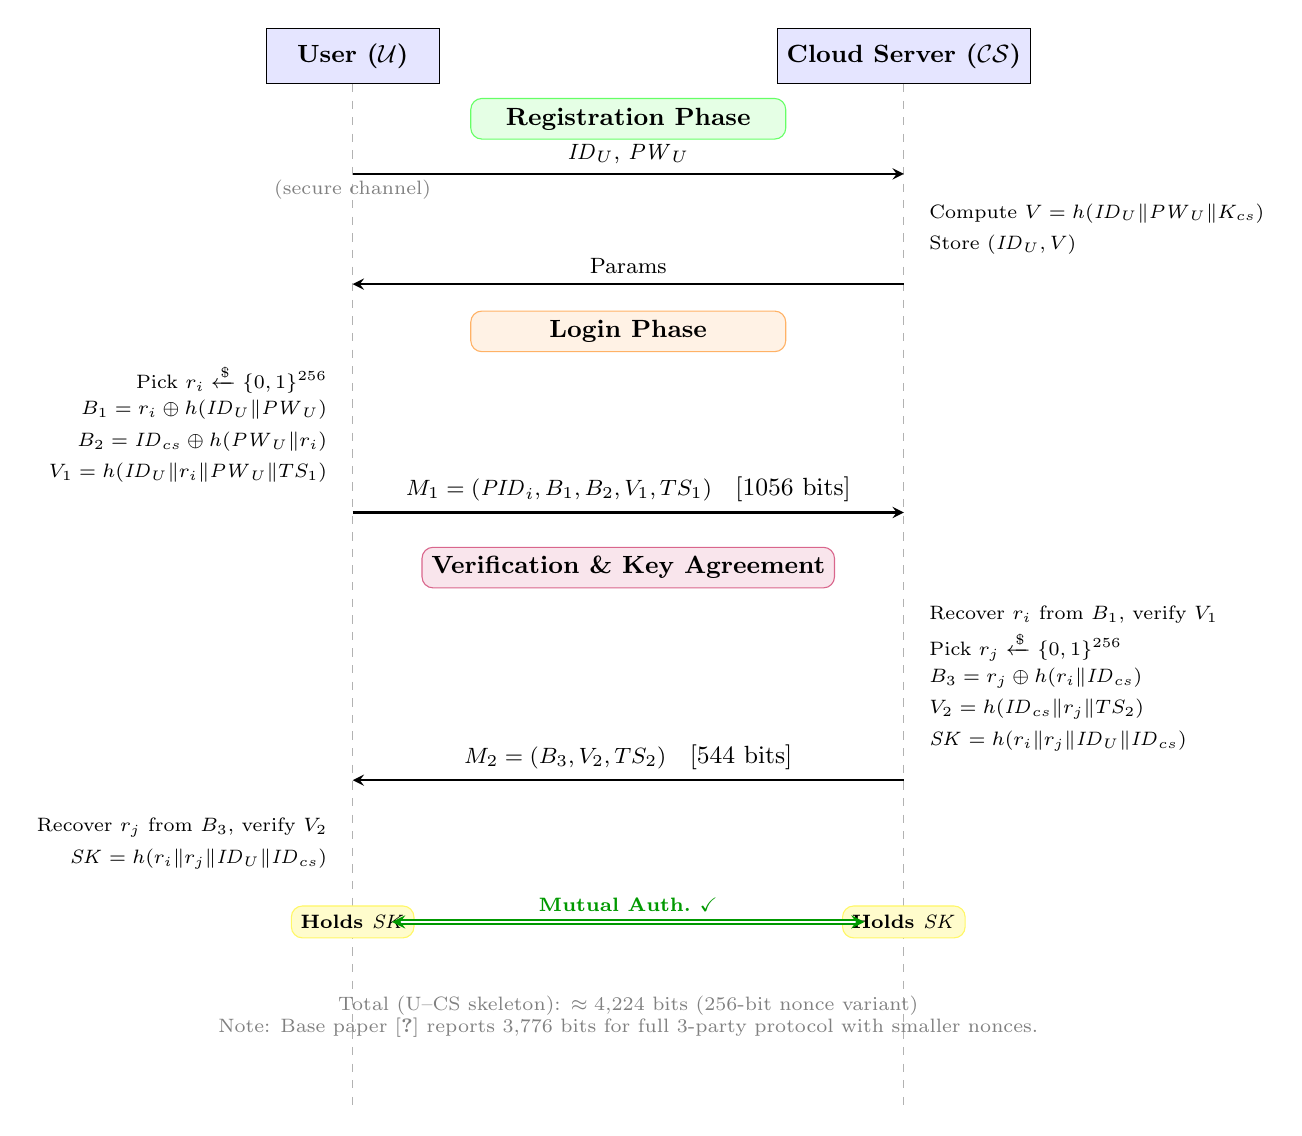
\begin{tikzpicture}[
  >=stealth,
  entity/.style={rectangle, draw, fill=blue!10, minimum width=2.2cm,
                 minimum height=0.7cm, font=\small\bfseries},
  msg/.style={->, thick},
  label/.style={font=\footnotesize, midway, above, sloped},
  note/.style={font=\scriptsize, text=gray}
]

% ---- Entities ----
\node[entity] (U)  at (0,0)    {User ($\mathcal{U}$)};
\node[entity] (CS) at (7,0)    {Cloud Server ($\mathcal{CS}$)};

% ---- Lifelines ----
\draw[dashed, gray!60] (U.south)  -- ++(0,-13);
\draw[dashed, gray!60] (CS.south) -- ++(0,-13);

% -------- REGISTRATION PHASE ---------
\node[font=\small\bfseries, fill=green!10, rounded corners, draw=green!60,
      minimum width=4cm] at (3.5,-0.8) {Registration Phase};

% Reg step 1: U -> CS
\draw[msg] (0,-1.5) -- (7,-1.5)
  node[label] {$\ID_U,\, \PW_U$};
\node[note] at (0,-1.7) {(secure channel)};

% CS computes V
\node[font=\scriptsize, align=left, anchor=west] at (7.2,-2.0)
  {Compute $V = h(\ID_U \| \PW_U \| K_{cs})$};
\node[font=\scriptsize, align=left, anchor=west] at (7.2,-2.4)
  {Store $(\ID_U, V)$};

% Reg step 2: CS -> U
\draw[msg] (7,-2.9) -- (0,-2.9)
  node[label] {$\text{Params}$};

% -------- LOGIN PHASE ---------
\node[font=\small\bfseries, fill=orange!10, rounded corners, draw=orange!60,
      minimum width=4cm] at (3.5,-3.5) {Login Phase};

% U computes M1
\node[font=\scriptsize, align=right, anchor=east] at (-0.2,-4.1)
  {Pick $r_i \xleftarrow{\$} \{0,1\}^{256}$};
\node[font=\scriptsize, align=right, anchor=east] at (-0.2,-4.5)
  {$B_1 = r_i \oplus h(\ID_U \| \PW_U)$};
\node[font=\scriptsize, align=right, anchor=east] at (-0.2,-4.9)
  {$B_2 = \ID_{cs} \oplus h(\PW_U \| r_i)$};
\node[font=\scriptsize, align=right, anchor=east] at (-0.2,-5.3)
  {$V_1 = h(\ID_U \| r_i \| \PW_U \| TS_1)$};

% M1: U -> CS
\draw[msg] (0,-5.8) -- (7,-5.8)
  node[label] {$M_1 = (\PID_i, B_1, B_2, V_1, TS_1)$\quad\small[1056 bits]};

% -------- VERIFICATION & KEY AGREEMENT PHASE ---------
\node[font=\small\bfseries, fill=purple!10, rounded corners, draw=purple!60,
      minimum width=4cm] at (3.5,-6.5) {Verification \& Key Agreement};

% CS verifies
\node[font=\scriptsize, align=left, anchor=west] at (7.2,-7.1)
  {Recover $r_i$ from $B_1$, verify $V_1$};
\node[font=\scriptsize, align=left, anchor=west] at (7.2,-7.5)
  {Pick $r_j \xleftarrow{\$} \{0,1\}^{256}$};
\node[font=\scriptsize, align=left, anchor=west] at (7.2,-7.9)
  {$B_3 = r_j \oplus h(r_i \| \ID_{cs})$};
\node[font=\scriptsize, align=left, anchor=west] at (7.2,-8.3)
  {$V_2 = h(\ID_{cs} \| r_j \| TS_2)$};
\node[font=\scriptsize, align=left, anchor=west] at (7.2,-8.7)
  {$\SK = h(r_i \| r_j \| \ID_U \| \ID_{cs})$};

% M2: CS -> U
\draw[msg] (7,-9.2) -- (0,-9.2)
  node[label] {$M_2 = (B_3, V_2, TS_2)$\quad\small[544 bits]};

% U derives SK
\node[font=\scriptsize, align=right, anchor=east] at (-0.2,-9.8)
  {Recover $r_j$ from $B_3$, verify $V_2$};
\node[font=\scriptsize, align=right, anchor=east] at (-0.2,-10.2)
  {$\SK = h(r_i \| r_j \| \ID_U \| \ID_{cs})$};

% Both hold SK
\node[font=\scriptsize\bfseries, fill=yellow!20, rounded corners, draw=yellow!60]
  at (0,-11.0) {Holds $\SK$};
\node[font=\scriptsize\bfseries, fill=yellow!20, rounded corners, draw=yellow!60]
  at (7,-11.0) {Holds $\SK$};
\draw[<->, double, thick, green!60!black] (0.5,-11.0) -- (6.5,-11.0)
  node[midway, above, font=\scriptsize\bfseries] {Mutual Auth.\ \checkmark};

% Communication overhead note
\node[note, align=center] at (3.5,-12.2)
  {Total (U--CS skeleton): $\approx 4{,}224$ bits (256-bit nonce variant)\\
   Note: Base paper \cite{JuPark2023} reports 3{,}776 bits for
   full 3-party protocol with smaller nonces.};

\end{tikzpicture}%
}
\caption{Message-flow diagram for the Hash+XOR mutual authentication scheme
(adapted from~\cite{JuPark2023}). This implementation covers the User--Cloud
leg only; the Control-Server leg and key-confirmation step are omitted from
the skeleton (see Section~\ref{sec:limitations}).
Total communication: 4,224 bits using 256-bit nonces throughout.}
\label{fig:hash_flow}
\end{figure*}

% =============================================================================
\begin{figure*}[!t]
\centering
\resizebox{0.92\textwidth}{!}{%
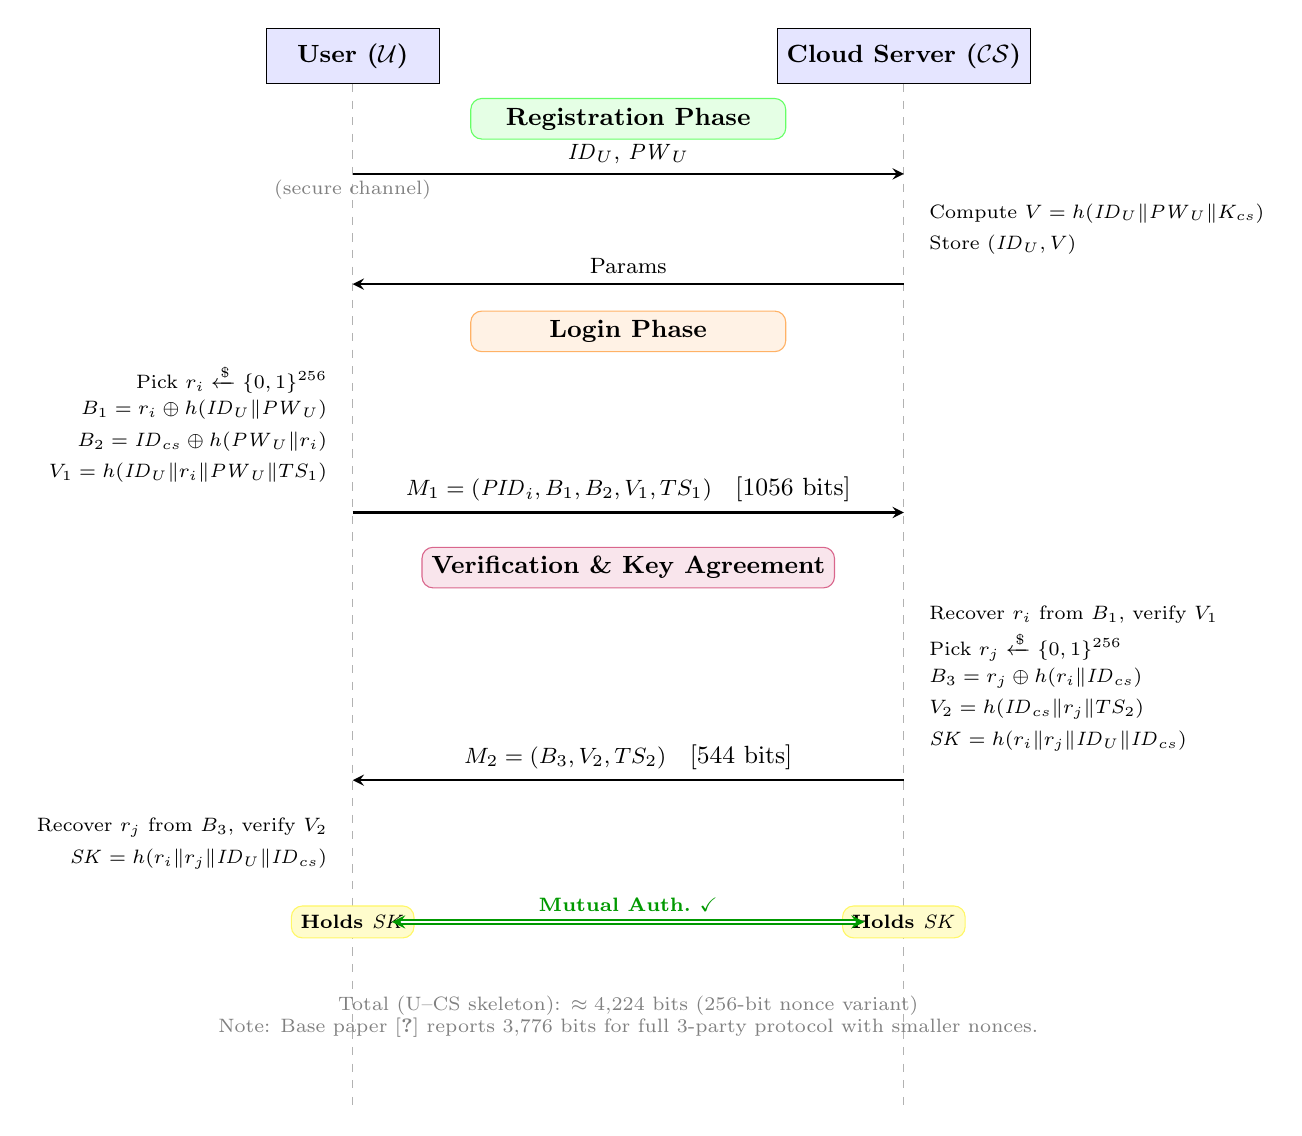
\begin{tikzpicture}[
  >=stealth,
  entity/.style={rectangle, draw, fill=blue!10, minimum width=2.2cm,
                 minimum height=0.7cm, font=\small\bfseries},
  msg/.style={->, thick},
  label/.style={font=\footnotesize, midway, above, sloped},
  note/.style={font=\scriptsize, text=gray}
]

% ---- Entities ----
\node[entity] (U)  at (0,0)    {User ($\mathcal{U}$)};
\node[entity] (CS) at (7,0)    {Cloud Server ($\mathcal{CS}$)};

% ---- Lifelines ----
\draw[dashed, gray!60] (U.south)  -- ++(0,-13);
\draw[dashed, gray!60] (CS.south) -- ++(0,-13);

% -------- REGISTRATION PHASE ---------
\node[font=\small\bfseries, fill=green!10, rounded corners, draw=green!60,
      minimum width=4cm] at (3.5,-0.8) {Registration Phase};

% Reg step 1: U -> CS
\draw[msg] (0,-1.5) -- (7,-1.5)
  node[label] {$\ID_U,\, \PW_U$};
\node[note] at (0,-1.7) {(secure channel)};

% CS computes V
\node[font=\scriptsize, align=left, anchor=west] at (7.2,-2.0)
  {Compute $V = h(\ID_U \| \PW_U \| K_{cs})$};
\node[font=\scriptsize, align=left, anchor=west] at (7.2,-2.4)
  {Store $(\ID_U, V)$};

% Reg step 2: CS -> U
\draw[msg] (7,-2.9) -- (0,-2.9)
  node[label] {$\text{Params}$};

% -------- LOGIN PHASE ---------
\node[font=\small\bfseries, fill=orange!10, rounded corners, draw=orange!60,
      minimum width=4cm] at (3.5,-3.5) {Login Phase};

% U computes M1
\node[font=\scriptsize, align=right, anchor=east] at (-0.2,-4.1)
  {Pick $r_i \xleftarrow{\$} \{0,1\}^{256}$};
\node[font=\scriptsize, align=right, anchor=east] at (-0.2,-4.5)
  {$B_1 = r_i \oplus h(\ID_U \| \PW_U)$};
\node[font=\scriptsize, align=right, anchor=east] at (-0.2,-4.9)
  {$B_2 = \ID_{cs} \oplus h(\PW_U \| r_i)$};
\node[font=\scriptsize, align=right, anchor=east] at (-0.2,-5.3)
  {$V_1 = h(\ID_U \| r_i \| \PW_U \| TS_1)$};

% M1: U -> CS
\draw[msg] (0,-5.8) -- (7,-5.8)
  node[label] {$M_1 = (\PID_i, B_1, B_2, V_1, TS_1)$\quad\small[1056 bits]};

% -------- VERIFICATION & KEY AGREEMENT PHASE ---------
\node[font=\small\bfseries, fill=purple!10, rounded corners, draw=purple!60,
      minimum width=4cm] at (3.5,-6.5) {Verification \& Key Agreement};

% CS verifies
\node[font=\scriptsize, align=left, anchor=west] at (7.2,-7.1)
  {Recover $r_i$ from $B_1$, verify $V_1$};
\node[font=\scriptsize, align=left, anchor=west] at (7.2,-7.5)
  {Pick $r_j \xleftarrow{\$} \{0,1\}^{256}$};
\node[font=\scriptsize, align=left, anchor=west] at (7.2,-7.9)
  {$B_3 = r_j \oplus h(r_i \| \ID_{cs})$};
\node[font=\scriptsize, align=left, anchor=west] at (7.2,-8.3)
  {$V_2 = h(\ID_{cs} \| r_j \| TS_2)$};
\node[font=\scriptsize, align=left, anchor=west] at (7.2,-8.7)
  {$\SK = h(r_i \| r_j \| \ID_U \| \ID_{cs})$};

% M2: CS -> U
\draw[msg] (7,-9.2) -- (0,-9.2)
  node[label] {$M_2 = (B_3, V_2, TS_2)$\quad\small[544 bits]};

% U derives SK
\node[font=\scriptsize, align=right, anchor=east] at (-0.2,-9.8)
  {Recover $r_j$ from $B_3$, verify $V_2$};
\node[font=\scriptsize, align=right, anchor=east] at (-0.2,-10.2)
  {$\SK = h(r_i \| r_j \| \ID_U \| \ID_{cs})$};

% Both hold SK
\node[font=\scriptsize\bfseries, fill=yellow!20, rounded corners, draw=yellow!60]
  at (0,-11.0) {Holds $\SK$};
\node[font=\scriptsize\bfseries, fill=yellow!20, rounded corners, draw=yellow!60]
  at (7,-11.0) {Holds $\SK$};
\draw[<->, double, thick, green!60!black] (0.5,-11.0) -- (6.5,-11.0)
  node[midway, above, font=\scriptsize\bfseries] {Mutual Auth.\ \checkmark};

% Communication overhead note
\node[note, align=center] at (3.5,-12.2)
  {Total (U--CS skeleton): $\approx 4{,}224$ bits (256-bit nonce variant)\\
   Note: Base paper \cite{JuPark2023} reports 3{,}776 bits for
   full 3-party protocol with smaller nonces.};

\end{tikzpicture}%
}
\caption{Message-flow diagram for the Hash+XOR mutual authentication scheme
(adapted from~\cite{JuPark2023}). This implementation covers the User--Cloud
leg only; the Control-Server leg and key-confirmation step are omitted from
the skeleton (see Section~\ref{sec:limitations}).
Total communication: 4,224 bits using 256-bit nonces throughout.}
\label{fig:hash_flow}
\end{figure*}

% =============================================================================
\begin{figure*}[!t]
\centering
\resizebox{0.92\textwidth}{!}{%
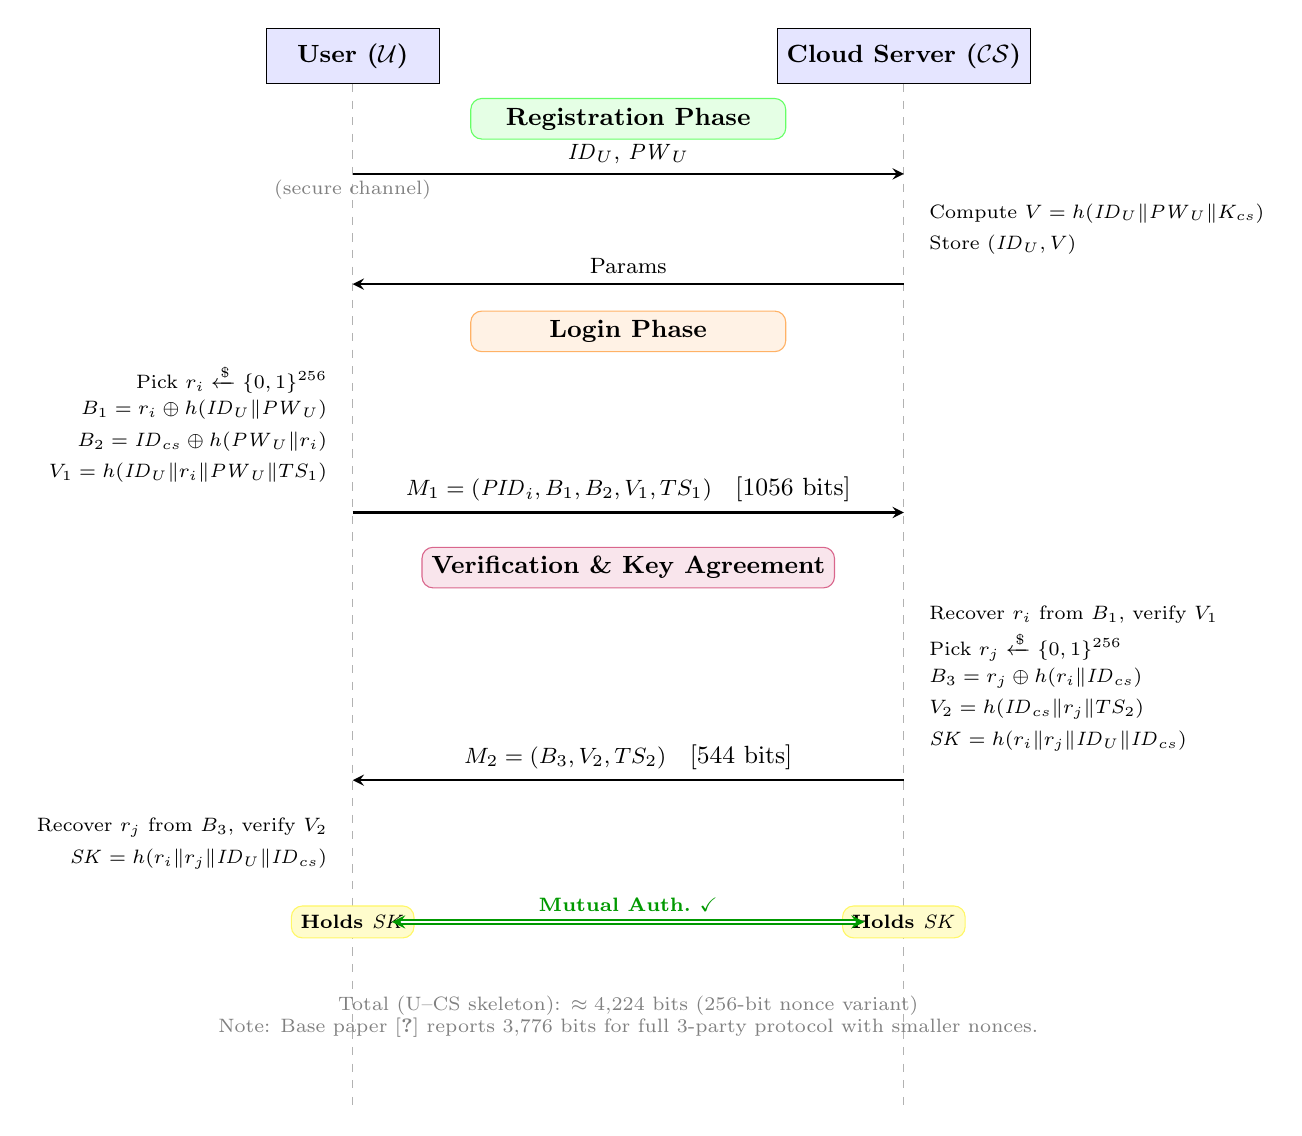
\begin{tikzpicture}[
  >=stealth,
  entity/.style={rectangle, draw, fill=blue!10, minimum width=2.2cm,
                 minimum height=0.7cm, font=\small\bfseries},
  msg/.style={->, thick},
  label/.style={font=\footnotesize, midway, above, sloped},
  note/.style={font=\scriptsize, text=gray}
]

% ---- Entities ----
\node[entity] (U)  at (0,0)    {User ($\mathcal{U}$)};
\node[entity] (CS) at (7,0)    {Cloud Server ($\mathcal{CS}$)};

% ---- Lifelines ----
\draw[dashed, gray!60] (U.south)  -- ++(0,-13);
\draw[dashed, gray!60] (CS.south) -- ++(0,-13);

% -------- REGISTRATION PHASE ---------
\node[font=\small\bfseries, fill=green!10, rounded corners, draw=green!60,
      minimum width=4cm] at (3.5,-0.8) {Registration Phase};

% Reg step 1: U -> CS
\draw[msg] (0,-1.5) -- (7,-1.5)
  node[label] {$\ID_U,\, \PW_U$};
\node[note] at (0,-1.7) {(secure channel)};

% CS computes V
\node[font=\scriptsize, align=left, anchor=west] at (7.2,-2.0)
  {Compute $V = h(\ID_U \| \PW_U \| K_{cs})$};
\node[font=\scriptsize, align=left, anchor=west] at (7.2,-2.4)
  {Store $(\ID_U, V)$};

% Reg step 2: CS -> U
\draw[msg] (7,-2.9) -- (0,-2.9)
  node[label] {$\text{Params}$};

% -------- LOGIN PHASE ---------
\node[font=\small\bfseries, fill=orange!10, rounded corners, draw=orange!60,
      minimum width=4cm] at (3.5,-3.5) {Login Phase};

% U computes M1
\node[font=\scriptsize, align=right, anchor=east] at (-0.2,-4.1)
  {Pick $r_i \xleftarrow{\$} \{0,1\}^{256}$};
\node[font=\scriptsize, align=right, anchor=east] at (-0.2,-4.5)
  {$B_1 = r_i \oplus h(\ID_U \| \PW_U)$};
\node[font=\scriptsize, align=right, anchor=east] at (-0.2,-4.9)
  {$B_2 = \ID_{cs} \oplus h(\PW_U \| r_i)$};
\node[font=\scriptsize, align=right, anchor=east] at (-0.2,-5.3)
  {$V_1 = h(\ID_U \| r_i \| \PW_U \| TS_1)$};

% M1: U -> CS
\draw[msg] (0,-5.8) -- (7,-5.8)
  node[label] {$M_1 = (\PID_i, B_1, B_2, V_1, TS_1)$\quad\small[1056 bits]};

% -------- VERIFICATION & KEY AGREEMENT PHASE ---------
\node[font=\small\bfseries, fill=purple!10, rounded corners, draw=purple!60,
      minimum width=4cm] at (3.5,-6.5) {Verification \& Key Agreement};

% CS verifies
\node[font=\scriptsize, align=left, anchor=west] at (7.2,-7.1)
  {Recover $r_i$ from $B_1$, verify $V_1$};
\node[font=\scriptsize, align=left, anchor=west] at (7.2,-7.5)
  {Pick $r_j \xleftarrow{\$} \{0,1\}^{256}$};
\node[font=\scriptsize, align=left, anchor=west] at (7.2,-7.9)
  {$B_3 = r_j \oplus h(r_i \| \ID_{cs})$};
\node[font=\scriptsize, align=left, anchor=west] at (7.2,-8.3)
  {$V_2 = h(\ID_{cs} \| r_j \| TS_2)$};
\node[font=\scriptsize, align=left, anchor=west] at (7.2,-8.7)
  {$\SK = h(r_i \| r_j \| \ID_U \| \ID_{cs})$};

% M2: CS -> U
\draw[msg] (7,-9.2) -- (0,-9.2)
  node[label] {$M_2 = (B_3, V_2, TS_2)$\quad\small[544 bits]};

% U derives SK
\node[font=\scriptsize, align=right, anchor=east] at (-0.2,-9.8)
  {Recover $r_j$ from $B_3$, verify $V_2$};
\node[font=\scriptsize, align=right, anchor=east] at (-0.2,-10.2)
  {$\SK = h(r_i \| r_j \| \ID_U \| \ID_{cs})$};

% Both hold SK
\node[font=\scriptsize\bfseries, fill=yellow!20, rounded corners, draw=yellow!60]
  at (0,-11.0) {Holds $\SK$};
\node[font=\scriptsize\bfseries, fill=yellow!20, rounded corners, draw=yellow!60]
  at (7,-11.0) {Holds $\SK$};
\draw[<->, double, thick, green!60!black] (0.5,-11.0) -- (6.5,-11.0)
  node[midway, above, font=\scriptsize\bfseries] {Mutual Auth.\ \checkmark};

% Communication overhead note
\node[note, align=center] at (3.5,-12.2)
  {Total (U--CS skeleton): $\approx 4{,}224$ bits (256-bit nonce variant)\\
   Note: Base paper \cite{JuPark2023} reports 3{,}776 bits for
   full 3-party protocol with smaller nonces.};

\end{tikzpicture}%
}
\caption{Message-flow diagram for the Hash+XOR mutual authentication scheme
(adapted from~\cite{JuPark2023}). This implementation covers the User--Cloud
leg only; the Control-Server leg and key-confirmation step are omitted from
the skeleton (see Section~\ref{sec:limitations}).
Total communication: 4,224 bits using 256-bit nonces throughout.}
\label{fig:hash_flow}
\end{figure*}


% =============================================================================
\section{ECC P-256 Counterpart}
\label{sec:ecc}

\subsection{Design Rationale}

The ECC counterpart replaces SHA-256+XOR key agreement with ephemeral
Elliptic-Curve Diffie-Hellman (ECDH) on the NIST P-256 curve and uses
a hash-based MAC for authentication. This design mirrors the structure of the
ephemeral (EC)DHE key exchange in TLS~1.3~\cite{RFC8446}. The primary
advantage is \emph{forward secrecy}: because ephemeral private keys are
erased at session end, a future compromise of long-term keys cannot recover
past session keys.

\subsection{Registration Phase}

Each party generates a long-term P-256 key pair; the User registers its
public key $Q_U$ with the Cloud Server, and the server returns $Q_S$.
No password or secret material is transmitted after this one-time step.

\subsection{Login and Key-Agreement Phase}

Algorithm~\ref{alg:ecc_login} describes the login and key-agreement
procedure.

\begin{algorithm}[!t]
\caption{ECC P-256 Login \& Key Agreement}
\label{alg:ecc_login}
\begin{algorithmic}[1]
\Require Long-term pairs $(d_U,\,Q_U)$ and $(d_S,\,Q_S)$; $G,\,n$ (P-256 params)
\Statex \textbf{--- User side ---}
\State Pick ephemeral $e_U \xleftarrow{\$} \mathbb{Z}_n^*$;
       compute $P_U = e_U \cdot G$
\State Pick nonce $N_i \xleftarrow{\$} \{0,1\}^{128}$
\State $V_i \leftarrow \h{\ID_U \| N_i \| P_U \| \TS_1}$
\State Send $M_1 = (P_U,\, N_i,\, \TS_1,\, V_i)$ to CS  \Comment{936 bits}
\Statex \textbf{--- Cloud Server side ---}
\State Check $|\text{now} - \TS_1| \leq \Delta T$; verify $V_i$; abort if not
\State Pick ephemeral $e_S \xleftarrow{\$} \mathbb{Z}_n^*$;
       compute $P_S = e_S \cdot G$
\State $Z \leftarrow e_S \cdot P_U$  \Comment{ECDH shared point, $x$-coord only}
\State Pick $N_c \xleftarrow{\$} \{0,1\}^{128}$
\State $\SK \leftarrow \h{Z \| N_i \| N_c \| \ID_U \| \ID_\CS}$
\State $V_j \leftarrow \h{\ID_\CS \| N_c \| P_S \| \SK \| \TS_2}$
\State Send $M_2 = (P_S,\, N_c,\, \TS_2,\, V_j)$ to User  \Comment{936 bits}
\Statex \textbf{--- User verifies ---}
\State $Z \leftarrow e_U \cdot P_S$  \Comment{Same ECDH point by commutativity}
\State $\SK \leftarrow \h{Z \| N_i \| N_c \| \ID_U \| \ID_\CS}$
\State Verify $V_j$; accept session if valid; \textbf{erase} $e_U$
\end{algorithmic}
\end{algorithm}

\subsection{Forward Secrecy Argument}

Because $e_U$ and $e_S$ are erased at the end of each session (line~14 of
Algorithm~\ref{alg:ecc_login}), $Z$ cannot be recomputed from any later state
information. An adversary who obtains long-term keys $d_U$ or $d_S$ after the
session cannot recover $Z$ and, therefore, cannot recover $\SK$. This is the
standard forward-secrecy argument for ephemeral ECDH~\cite{RFC8446}.

The message-flow is illustrated in Fig.~\ref{fig:ecc_flow}.

% =============================================================================
% fig_ecc_flow.tex  —  TikZ sequence diagram for ECC P-256 counterpart
% Include in main.tex with:  % =============================================================================
% fig_ecc_flow.tex  —  TikZ sequence diagram for ECC P-256 counterpart
% Include in main.tex with:  % =============================================================================
% fig_ecc_flow.tex  —  TikZ sequence diagram for ECC P-256 counterpart
% Include in main.tex with:  \input{figures/fig_ecc_flow}
% =============================================================================
\begin{figure*}[!t]
\centering
\resizebox{0.92\textwidth}{!}{%
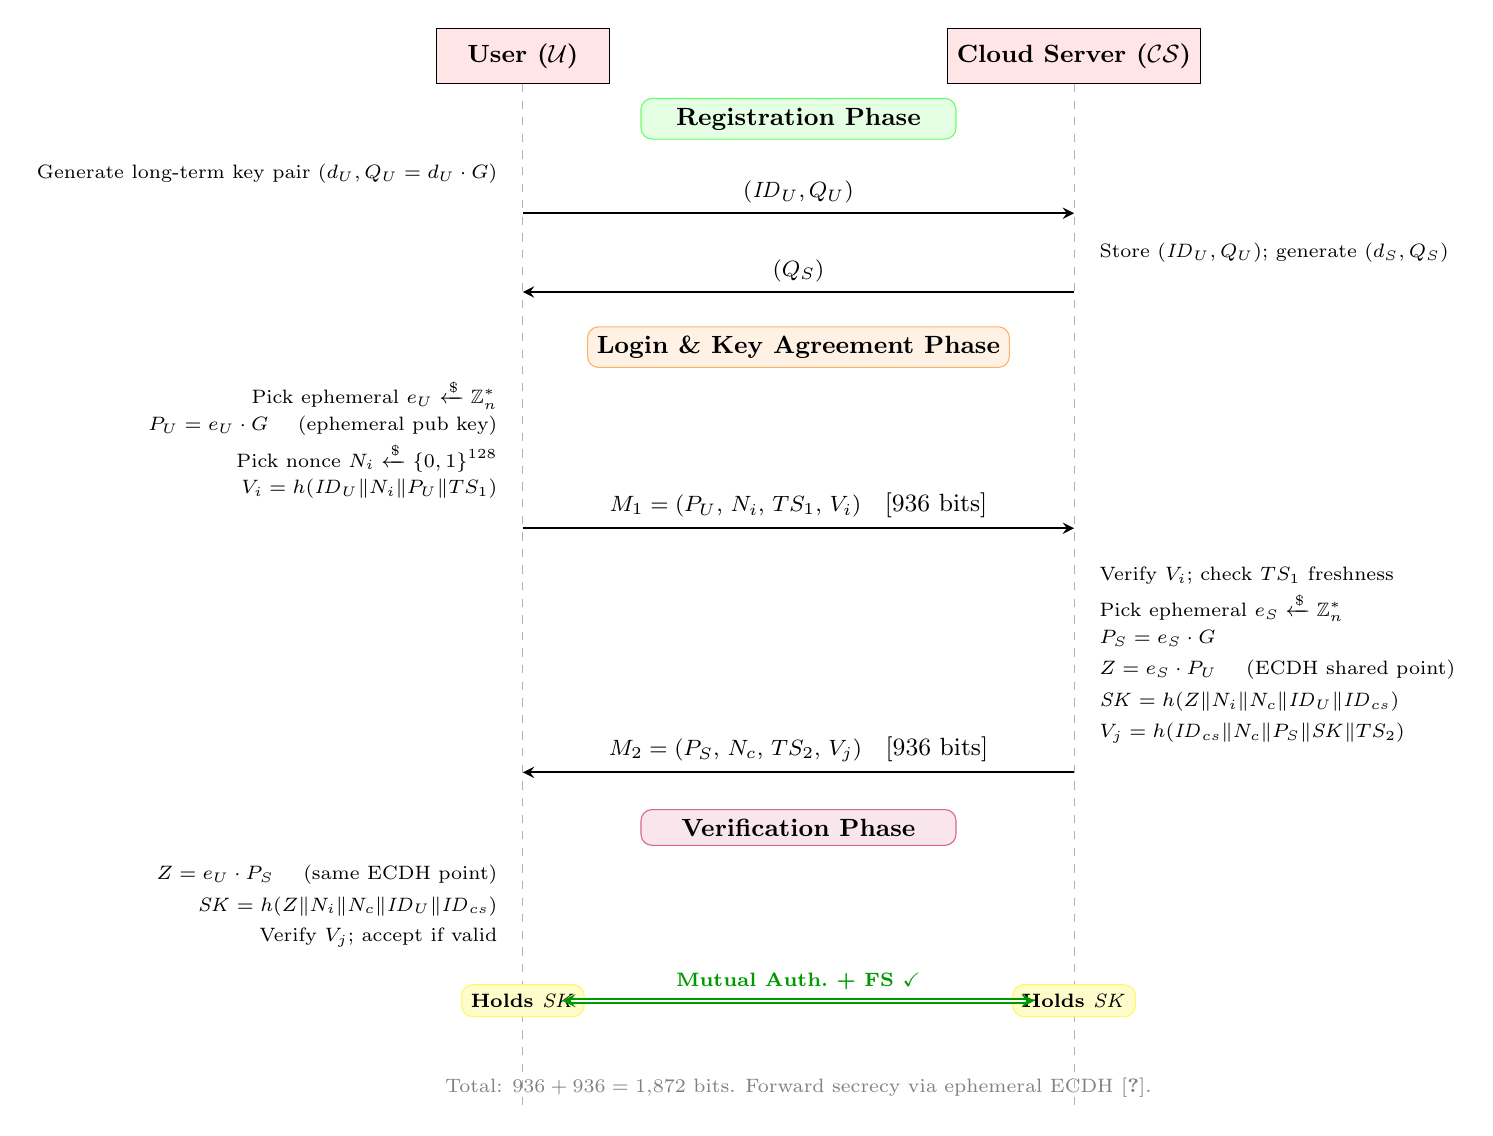
\begin{tikzpicture}[
  >=stealth,
  entity/.style={rectangle, draw, fill=red!10, minimum width=2.2cm,
                 minimum height=0.7cm, font=\small\bfseries},
  msg/.style={->, thick},
  label/.style={font=\footnotesize, midway, above, sloped},
  note/.style={font=\scriptsize, text=gray}
]

% ---- Entities ----
\node[entity] (U)  at (0,0)    {User ($\mathcal{U}$)};
\node[entity] (CS) at (7,0)    {Cloud Server ($\mathcal{CS}$)};

% ---- Lifelines ----
\draw[dashed, gray!60] (U.south)  -- ++(0,-13);
\draw[dashed, gray!60] (CS.south) -- ++(0,-13);

% -------- REGISTRATION PHASE ---------
\node[font=\small\bfseries, fill=green!10, rounded corners, draw=green!60,
      minimum width=4cm] at (3.5,-0.8) {Registration Phase};

\node[font=\scriptsize, align=right, anchor=east] at (-0.2,-1.5)
  {Generate long-term key pair $(d_U, Q_U = d_U \cdot G)$};
% U -> CS
\draw[msg] (0,-2.0) -- (7,-2.0)
  node[label] {$(\ID_U, Q_U)$};
\node[font=\scriptsize, align=left, anchor=west] at (7.2,-2.5)
  {Store $(\ID_U, Q_U)$; generate $(d_S, Q_S)$};
% CS -> U
\draw[msg] (7,-3.0) -- (0,-3.0)
  node[label] {$(Q_S)$};

% -------- LOGIN \& KEY AGREEMENT PHASE ---------
\node[font=\small\bfseries, fill=orange!10, rounded corners, draw=orange!60,
      minimum width=4cm] at (3.5,-3.7) {Login \& Key Agreement Phase};

% U side computations
\node[font=\scriptsize, align=right, anchor=east] at (-0.2,-4.3)
  {Pick ephemeral $e_U \xleftarrow{\$} \mathbb{Z}_n^*$};
\node[font=\scriptsize, align=right, anchor=east] at (-0.2,-4.7)
  {$P_U = e_U \cdot G$ \quad (ephemeral pub key)};
\node[font=\scriptsize, align=right, anchor=east] at (-0.2,-5.1)
  {Pick nonce $N_i \xleftarrow{\$} \{0,1\}^{128}$};
\node[font=\scriptsize, align=right, anchor=east] at (-0.2,-5.5)
  {$V_i = h(\ID_U \| N_i \| P_U \| TS_1)$};

% M1: U -> CS   [936 bits]
\draw[msg] (0,-6.0) -- (7,-6.0)
  node[label] {$M_1 = (P_U,\, N_i,\, TS_1,\, V_i)$\quad\small[936 bits]};

% CS side
\node[font=\scriptsize, align=left, anchor=west] at (7.2,-6.6)
  {Verify $V_i$; check $TS_1$ freshness};
\node[font=\scriptsize, align=left, anchor=west] at (7.2,-7.0)
  {Pick ephemeral $e_S \xleftarrow{\$} \mathbb{Z}_n^*$};
\node[font=\scriptsize, align=left, anchor=west] at (7.2,-7.4)
  {$P_S = e_S \cdot G$};
\node[font=\scriptsize, align=left, anchor=west] at (7.2,-7.8)
  {$Z = e_S \cdot P_U$ \quad (ECDH shared point)};
\node[font=\scriptsize, align=left, anchor=west] at (7.2,-8.2)
  {$\SK = h(Z \| N_i \| N_c \| \ID_U \| \ID_{cs})$};
\node[font=\scriptsize, align=left, anchor=west] at (7.2,-8.6)
  {$V_j = h(\ID_{cs} \| N_c \| P_S \| \SK \| TS_2)$};

% M2: CS -> U   [936 bits]
\draw[msg] (7,-9.1) -- (0,-9.1)
  node[label] {$M_2 = (P_S,\, N_c,\, TS_2,\, V_j)$\quad\small[936 bits]};

% -------- VERIFICATION ---------
\node[font=\small\bfseries, fill=purple!10, rounded corners, draw=purple!60,
      minimum width=4cm] at (3.5,-9.8) {Verification Phase};

\node[font=\scriptsize, align=right, anchor=east] at (-0.2,-10.4)
  {$Z = e_U \cdot P_S$ \quad (same ECDH point)};
\node[font=\scriptsize, align=right, anchor=east] at (-0.2,-10.8)
  {$\SK = h(Z \| N_i \| N_c \| \ID_U \| \ID_{cs})$};
\node[font=\scriptsize, align=right, anchor=east] at (-0.2,-11.2)
  {Verify $V_j$; accept if valid};

% Both hold SK
\node[font=\scriptsize\bfseries, fill=yellow!20, rounded corners, draw=yellow!60]
  at (0,-12.0) {Holds $\SK$};
\node[font=\scriptsize\bfseries, fill=yellow!20, rounded corners, draw=yellow!60]
  at (7,-12.0) {Holds $\SK$};
\draw[<->, double, thick, green!60!black] (0.5,-12.0) -- (6.5,-12.0)
  node[midway, above, font=\scriptsize\bfseries] {Mutual Auth.\ + FS \checkmark};

% Communication note
\node[note, align=center] at (3.5,-13.1)
  {Total: $936 + 936 = 1{,}872$ bits.
   Forward secrecy via ephemeral ECDH~\cite{RFC8446}.};

\end{tikzpicture}%
}
\caption{Message-flow diagram for the ECC P-256 counterpart protocol.
Ephemeral ECDH key pairs $(e_U, P_U)$ and $(e_S, P_S)$ are discarded after
each session, providing forward secrecy. Total communication overhead is
1,872 bits, approximately 2.3$\times$ lower than the Hash+XOR skeleton
(4,224 bits) due to the use of compact nonces.}
\label{fig:ecc_flow}
\end{figure*}

% =============================================================================
\begin{figure*}[!t]
\centering
\resizebox{0.92\textwidth}{!}{%
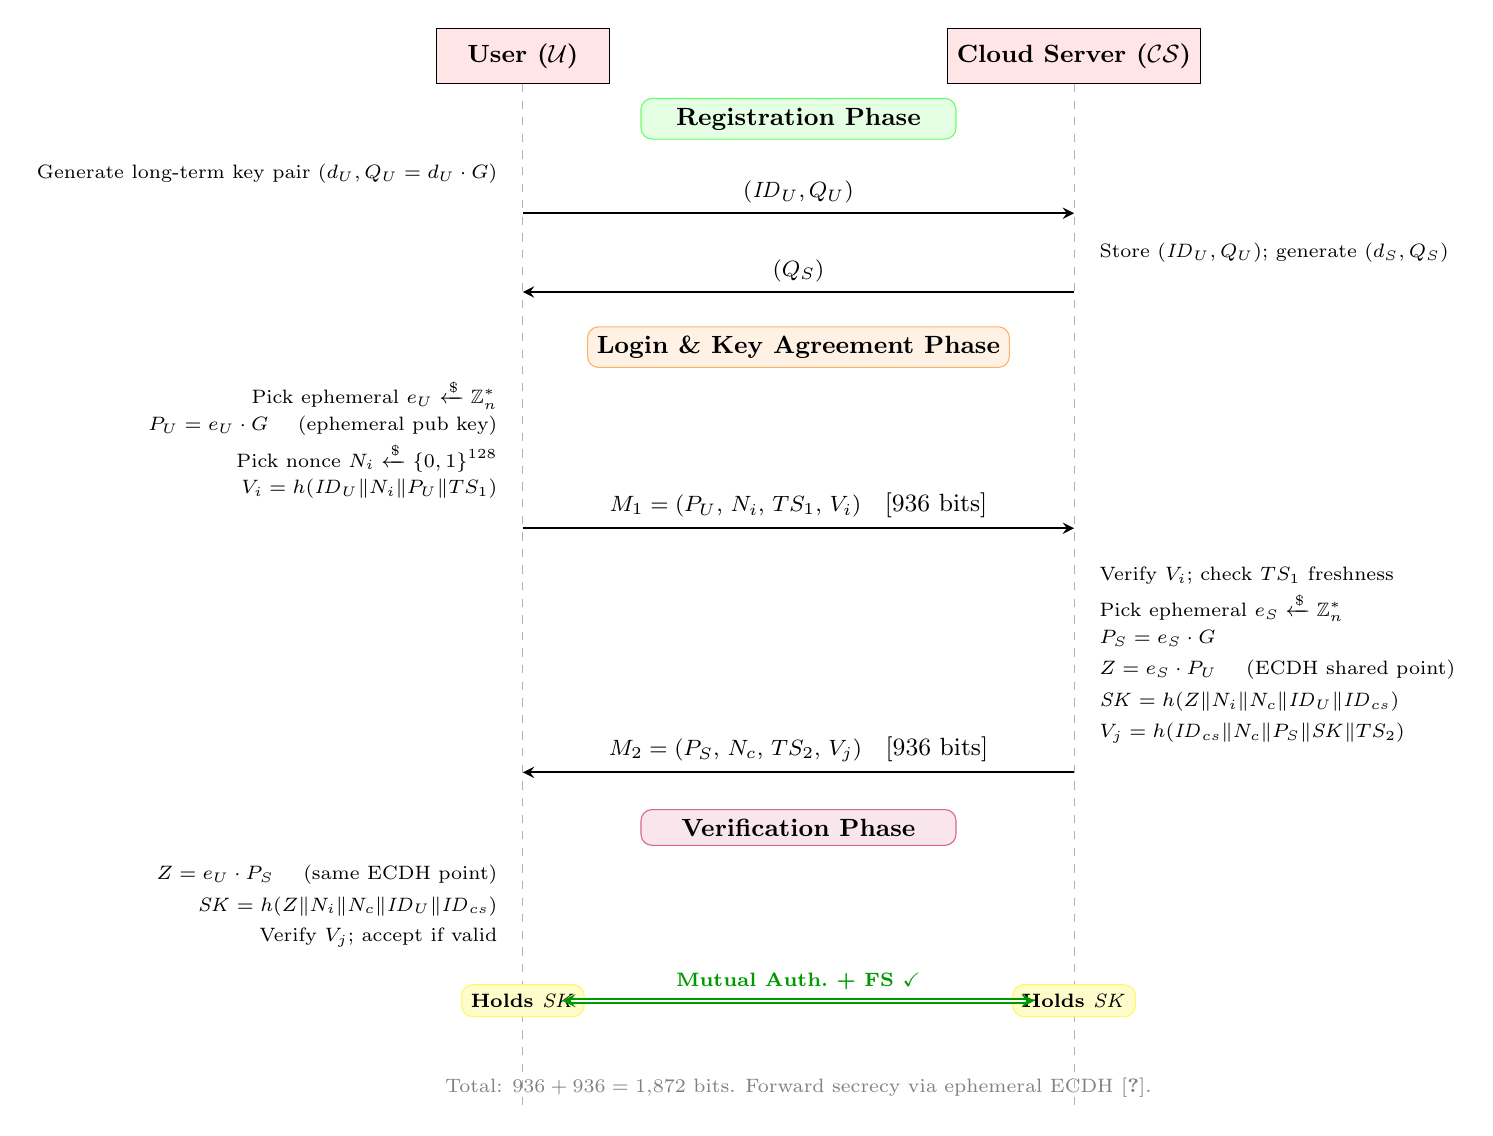
\begin{tikzpicture}[
  >=stealth,
  entity/.style={rectangle, draw, fill=red!10, minimum width=2.2cm,
                 minimum height=0.7cm, font=\small\bfseries},
  msg/.style={->, thick},
  label/.style={font=\footnotesize, midway, above, sloped},
  note/.style={font=\scriptsize, text=gray}
]

% ---- Entities ----
\node[entity] (U)  at (0,0)    {User ($\mathcal{U}$)};
\node[entity] (CS) at (7,0)    {Cloud Server ($\mathcal{CS}$)};

% ---- Lifelines ----
\draw[dashed, gray!60] (U.south)  -- ++(0,-13);
\draw[dashed, gray!60] (CS.south) -- ++(0,-13);

% -------- REGISTRATION PHASE ---------
\node[font=\small\bfseries, fill=green!10, rounded corners, draw=green!60,
      minimum width=4cm] at (3.5,-0.8) {Registration Phase};

\node[font=\scriptsize, align=right, anchor=east] at (-0.2,-1.5)
  {Generate long-term key pair $(d_U, Q_U = d_U \cdot G)$};
% U -> CS
\draw[msg] (0,-2.0) -- (7,-2.0)
  node[label] {$(\ID_U, Q_U)$};
\node[font=\scriptsize, align=left, anchor=west] at (7.2,-2.5)
  {Store $(\ID_U, Q_U)$; generate $(d_S, Q_S)$};
% CS -> U
\draw[msg] (7,-3.0) -- (0,-3.0)
  node[label] {$(Q_S)$};

% -------- LOGIN \& KEY AGREEMENT PHASE ---------
\node[font=\small\bfseries, fill=orange!10, rounded corners, draw=orange!60,
      minimum width=4cm] at (3.5,-3.7) {Login \& Key Agreement Phase};

% U side computations
\node[font=\scriptsize, align=right, anchor=east] at (-0.2,-4.3)
  {Pick ephemeral $e_U \xleftarrow{\$} \mathbb{Z}_n^*$};
\node[font=\scriptsize, align=right, anchor=east] at (-0.2,-4.7)
  {$P_U = e_U \cdot G$ \quad (ephemeral pub key)};
\node[font=\scriptsize, align=right, anchor=east] at (-0.2,-5.1)
  {Pick nonce $N_i \xleftarrow{\$} \{0,1\}^{128}$};
\node[font=\scriptsize, align=right, anchor=east] at (-0.2,-5.5)
  {$V_i = h(\ID_U \| N_i \| P_U \| TS_1)$};

% M1: U -> CS   [936 bits]
\draw[msg] (0,-6.0) -- (7,-6.0)
  node[label] {$M_1 = (P_U,\, N_i,\, TS_1,\, V_i)$\quad\small[936 bits]};

% CS side
\node[font=\scriptsize, align=left, anchor=west] at (7.2,-6.6)
  {Verify $V_i$; check $TS_1$ freshness};
\node[font=\scriptsize, align=left, anchor=west] at (7.2,-7.0)
  {Pick ephemeral $e_S \xleftarrow{\$} \mathbb{Z}_n^*$};
\node[font=\scriptsize, align=left, anchor=west] at (7.2,-7.4)
  {$P_S = e_S \cdot G$};
\node[font=\scriptsize, align=left, anchor=west] at (7.2,-7.8)
  {$Z = e_S \cdot P_U$ \quad (ECDH shared point)};
\node[font=\scriptsize, align=left, anchor=west] at (7.2,-8.2)
  {$\SK = h(Z \| N_i \| N_c \| \ID_U \| \ID_{cs})$};
\node[font=\scriptsize, align=left, anchor=west] at (7.2,-8.6)
  {$V_j = h(\ID_{cs} \| N_c \| P_S \| \SK \| TS_2)$};

% M2: CS -> U   [936 bits]
\draw[msg] (7,-9.1) -- (0,-9.1)
  node[label] {$M_2 = (P_S,\, N_c,\, TS_2,\, V_j)$\quad\small[936 bits]};

% -------- VERIFICATION ---------
\node[font=\small\bfseries, fill=purple!10, rounded corners, draw=purple!60,
      minimum width=4cm] at (3.5,-9.8) {Verification Phase};

\node[font=\scriptsize, align=right, anchor=east] at (-0.2,-10.4)
  {$Z = e_U \cdot P_S$ \quad (same ECDH point)};
\node[font=\scriptsize, align=right, anchor=east] at (-0.2,-10.8)
  {$\SK = h(Z \| N_i \| N_c \| \ID_U \| \ID_{cs})$};
\node[font=\scriptsize, align=right, anchor=east] at (-0.2,-11.2)
  {Verify $V_j$; accept if valid};

% Both hold SK
\node[font=\scriptsize\bfseries, fill=yellow!20, rounded corners, draw=yellow!60]
  at (0,-12.0) {Holds $\SK$};
\node[font=\scriptsize\bfseries, fill=yellow!20, rounded corners, draw=yellow!60]
  at (7,-12.0) {Holds $\SK$};
\draw[<->, double, thick, green!60!black] (0.5,-12.0) -- (6.5,-12.0)
  node[midway, above, font=\scriptsize\bfseries] {Mutual Auth.\ + FS \checkmark};

% Communication note
\node[note, align=center] at (3.5,-13.1)
  {Total: $936 + 936 = 1{,}872$ bits.
   Forward secrecy via ephemeral ECDH~\cite{RFC8446}.};

\end{tikzpicture}%
}
\caption{Message-flow diagram for the ECC P-256 counterpart protocol.
Ephemeral ECDH key pairs $(e_U, P_U)$ and $(e_S, P_S)$ are discarded after
each session, providing forward secrecy. Total communication overhead is
1,872 bits, approximately 2.3$\times$ lower than the Hash+XOR skeleton
(4,224 bits) due to the use of compact nonces.}
\label{fig:ecc_flow}
\end{figure*}

% =============================================================================
\begin{figure*}[!t]
\centering
\resizebox{0.92\textwidth}{!}{%
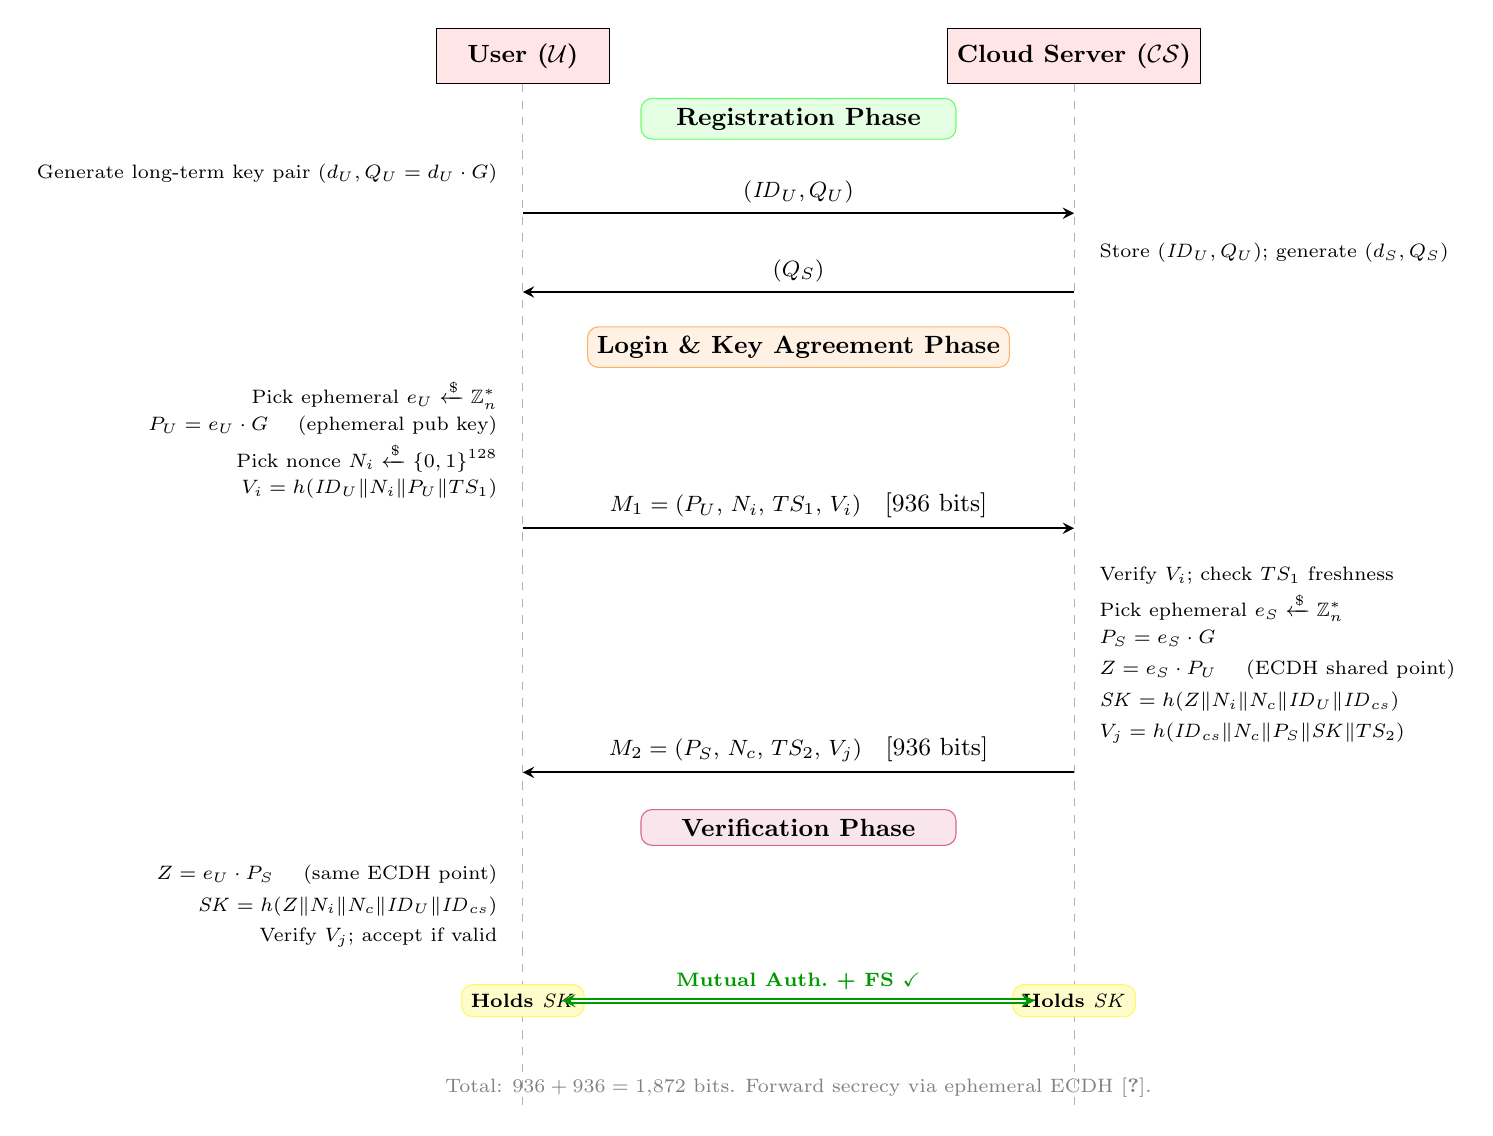
\begin{tikzpicture}[
  >=stealth,
  entity/.style={rectangle, draw, fill=red!10, minimum width=2.2cm,
                 minimum height=0.7cm, font=\small\bfseries},
  msg/.style={->, thick},
  label/.style={font=\footnotesize, midway, above, sloped},
  note/.style={font=\scriptsize, text=gray}
]

% ---- Entities ----
\node[entity] (U)  at (0,0)    {User ($\mathcal{U}$)};
\node[entity] (CS) at (7,0)    {Cloud Server ($\mathcal{CS}$)};

% ---- Lifelines ----
\draw[dashed, gray!60] (U.south)  -- ++(0,-13);
\draw[dashed, gray!60] (CS.south) -- ++(0,-13);

% -------- REGISTRATION PHASE ---------
\node[font=\small\bfseries, fill=green!10, rounded corners, draw=green!60,
      minimum width=4cm] at (3.5,-0.8) {Registration Phase};

\node[font=\scriptsize, align=right, anchor=east] at (-0.2,-1.5)
  {Generate long-term key pair $(d_U, Q_U = d_U \cdot G)$};
% U -> CS
\draw[msg] (0,-2.0) -- (7,-2.0)
  node[label] {$(\ID_U, Q_U)$};
\node[font=\scriptsize, align=left, anchor=west] at (7.2,-2.5)
  {Store $(\ID_U, Q_U)$; generate $(d_S, Q_S)$};
% CS -> U
\draw[msg] (7,-3.0) -- (0,-3.0)
  node[label] {$(Q_S)$};

% -------- LOGIN \& KEY AGREEMENT PHASE ---------
\node[font=\small\bfseries, fill=orange!10, rounded corners, draw=orange!60,
      minimum width=4cm] at (3.5,-3.7) {Login \& Key Agreement Phase};

% U side computations
\node[font=\scriptsize, align=right, anchor=east] at (-0.2,-4.3)
  {Pick ephemeral $e_U \xleftarrow{\$} \mathbb{Z}_n^*$};
\node[font=\scriptsize, align=right, anchor=east] at (-0.2,-4.7)
  {$P_U = e_U \cdot G$ \quad (ephemeral pub key)};
\node[font=\scriptsize, align=right, anchor=east] at (-0.2,-5.1)
  {Pick nonce $N_i \xleftarrow{\$} \{0,1\}^{128}$};
\node[font=\scriptsize, align=right, anchor=east] at (-0.2,-5.5)
  {$V_i = h(\ID_U \| N_i \| P_U \| TS_1)$};

% M1: U -> CS   [936 bits]
\draw[msg] (0,-6.0) -- (7,-6.0)
  node[label] {$M_1 = (P_U,\, N_i,\, TS_1,\, V_i)$\quad\small[936 bits]};

% CS side
\node[font=\scriptsize, align=left, anchor=west] at (7.2,-6.6)
  {Verify $V_i$; check $TS_1$ freshness};
\node[font=\scriptsize, align=left, anchor=west] at (7.2,-7.0)
  {Pick ephemeral $e_S \xleftarrow{\$} \mathbb{Z}_n^*$};
\node[font=\scriptsize, align=left, anchor=west] at (7.2,-7.4)
  {$P_S = e_S \cdot G$};
\node[font=\scriptsize, align=left, anchor=west] at (7.2,-7.8)
  {$Z = e_S \cdot P_U$ \quad (ECDH shared point)};
\node[font=\scriptsize, align=left, anchor=west] at (7.2,-8.2)
  {$\SK = h(Z \| N_i \| N_c \| \ID_U \| \ID_{cs})$};
\node[font=\scriptsize, align=left, anchor=west] at (7.2,-8.6)
  {$V_j = h(\ID_{cs} \| N_c \| P_S \| \SK \| TS_2)$};

% M2: CS -> U   [936 bits]
\draw[msg] (7,-9.1) -- (0,-9.1)
  node[label] {$M_2 = (P_S,\, N_c,\, TS_2,\, V_j)$\quad\small[936 bits]};

% -------- VERIFICATION ---------
\node[font=\small\bfseries, fill=purple!10, rounded corners, draw=purple!60,
      minimum width=4cm] at (3.5,-9.8) {Verification Phase};

\node[font=\scriptsize, align=right, anchor=east] at (-0.2,-10.4)
  {$Z = e_U \cdot P_S$ \quad (same ECDH point)};
\node[font=\scriptsize, align=right, anchor=east] at (-0.2,-10.8)
  {$\SK = h(Z \| N_i \| N_c \| \ID_U \| \ID_{cs})$};
\node[font=\scriptsize, align=right, anchor=east] at (-0.2,-11.2)
  {Verify $V_j$; accept if valid};

% Both hold SK
\node[font=\scriptsize\bfseries, fill=yellow!20, rounded corners, draw=yellow!60]
  at (0,-12.0) {Holds $\SK$};
\node[font=\scriptsize\bfseries, fill=yellow!20, rounded corners, draw=yellow!60]
  at (7,-12.0) {Holds $\SK$};
\draw[<->, double, thick, green!60!black] (0.5,-12.0) -- (6.5,-12.0)
  node[midway, above, font=\scriptsize\bfseries] {Mutual Auth.\ + FS \checkmark};

% Communication note
\node[note, align=center] at (3.5,-13.1)
  {Total: $936 + 936 = 1{,}872$ bits.
   Forward secrecy via ephemeral ECDH~\cite{RFC8446}.};

\end{tikzpicture}%
}
\caption{Message-flow diagram for the ECC P-256 counterpart protocol.
Ephemeral ECDH key pairs $(e_U, P_U)$ and $(e_S, P_S)$ are discarded after
each session, providing forward secrecy. Total communication overhead is
1,872 bits, approximately 2.3$\times$ lower than the Hash+XOR skeleton
(4,224 bits) due to the use of compact nonces.}
\label{fig:ecc_flow}
\end{figure*}


% =============================================================================
\section{Security Analysis}
\label{sec:security}

\subsection{Methodology and Limitations}

The security evaluation presented here is \emph{informal}: we model each
attack as a Python test case, execute it against the live protocol
implementation, and record whether the attack is detected. This approach
demonstrates concrete resistance under the implemented logic but does
\textbf{not} constitute a formal cryptographic proof. Formal analysis using
ProVerif~\cite{Blanchet2016} or Tamarin~\cite{Meieretal2013} is identified
as future work (Section~\ref{sec:conclusion}).

\subsection{Attack Tests}

\textbf{A1~-- Replay Attack.}
An adversary $\adv$ intercepts and re-sends a previously observed message
$M_1$ from an earlier session. Both protocols include a timestamp $\TS$ in
the authenticated payload and reject any message with
$|\text{now} - \TS| > \Delta T$ (set to 30~s in our implementation).
\emph{Result}: Both schemes \textbf{pass}; the replayed message is detected
and rejected.

\textbf{A2~-- Delayed Replay Attack.}
$\adv$ replays $M_1$ after more than $\Delta T$ seconds have elapsed.
The timestamp check directly rejects such messages.
\emph{Result}: Both schemes \textbf{pass}.

\textbf{A3~-- MITM / Tamper Attack.}
$\adv$ intercepts $M_1$ and flips one or more bits before forwarding it.
The HMAC/hash authenticator ($V_1$ or $V_i$) covers the entire message
payload; any bitflip produces a verification failure.
\emph{Result}: Both schemes \textbf{pass}; tampered messages are rejected at
the verification step.

\textbf{A4~-- Impersonation Attack.}
$\adv$ attempts to impersonate the User by constructing a fresh $M_1$
without knowledge of $\PW_U$ (hash+XOR scheme) or $d_U$ (ECC scheme).
Without the secret material, $\adv$ cannot compute a valid authenticator
$V_1$/$V_i$ that passes verification.
\emph{Result}: Both schemes \textbf{pass}.

\subsection{Security Property Comparison}

Fig.~\ref{fig:security_matrix} summarises the security properties of both
protocols.

% =============================================================================
% fig_security_matrix.tex  —  TikZ security property comparison matrix
% Scaled with \resizebox to strictly fit within \columnwidth in both
% two-column and single-column modes without overlapping adjacent text.
% Include with:  % =============================================================================
% fig_security_matrix.tex  —  TikZ security property comparison matrix
% Scaled with \resizebox to strictly fit within \columnwidth in both
% two-column and single-column modes without overlapping adjacent text.
% Include with:  % =============================================================================
% fig_security_matrix.tex  —  TikZ security property comparison matrix
% Scaled with \resizebox to strictly fit within \columnwidth in both
% two-column and single-column modes without overlapping adjacent text.
% Include with:  \input{figures/fig_security_matrix}
% =============================================================================
\begin{figure}[!t]
\centering
\resizebox{\columnwidth}{!}{%
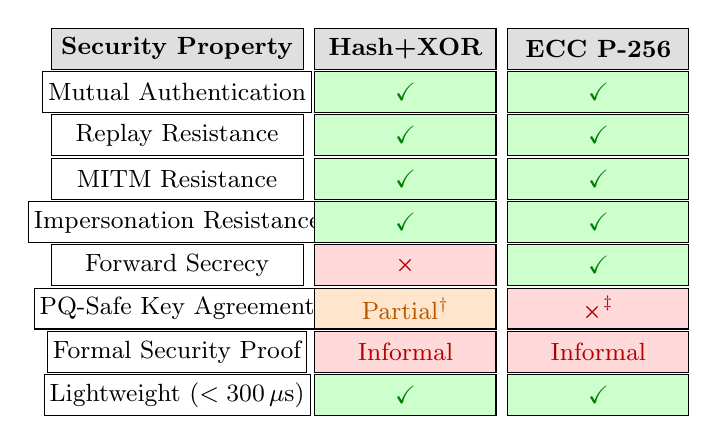
\begin{tikzpicture}[
  font=\small,
  cell/.style={draw, minimum width=2.3cm, minimum height=0.52cm,
               inner sep=2pt, align=center},
  header/.style={cell, fill=gray!25, font=\small\bfseries},
  yes/.style={cell, fill=green!20, text=green!50!black},
  no/.style={cell, fill=red!15, text=red!70!black},
  partial/.style={cell, fill=orange!20, text=orange!70!black},
]
% ---- Header row ----
\node[header, minimum width=3.2cm] (h0) at (0,0) {Security Property};
\node[header] (h1) at (2.9,0) {Hash+XOR};
\node[header] (h2) at (5.35,0) {ECC P-256};

% ---- Row 1: Mutual Authentication ----
\node[cell, minimum width=3.2cm] at (0,-0.55) {Mutual Authentication};
\node[yes]  at (2.9,-0.55) {\checkmark};
\node[yes]  at (5.35,-0.55) {\checkmark};

% ---- Row 2: Replay Resistance ----
\node[cell, minimum width=3.2cm] at (0,-1.1) {Replay Resistance};
\node[yes]  at (2.9,-1.1) {\checkmark};
\node[yes]  at (5.35,-1.1) {\checkmark};

% ---- Row 3: MITM / Tampering Resistance ----
\node[cell, minimum width=3.2cm] at (0,-1.65) {MITM Resistance};
\node[yes]  at (2.9,-1.65) {\checkmark};
\node[yes]  at (5.35,-1.65) {\checkmark};

% ---- Row 4: Impersonation Resistance ----
\node[cell, minimum width=3.2cm] at (0,-2.2) {Impersonation Resistance};
\node[yes]  at (2.9,-2.2) {\checkmark};
\node[yes]  at (5.35,-2.2) {\checkmark};

% ---- Row 5: Forward Secrecy ----
\node[cell, minimum width=3.2cm] at (0,-2.75) {Forward Secrecy};
\node[no]   at (2.9,-2.75) {\texttimes};
\node[yes]  at (5.35,-2.75) {\checkmark};

% ---- Row 6: PQ-Safe Key Agreement ----
\node[cell, minimum width=3.2cm] at (0,-3.3) {PQ-Safe Key Agreement};
\node[partial] at (2.9,-3.3) {Partial$^\dagger$};
\node[no]   at (5.35,-3.3) {\texttimes$^\ddagger$};

% ---- Row 7: Formal Security Proof ----
\node[cell, minimum width=3.2cm] at (0,-3.85) {Formal Security Proof};
\node[no]   at (2.9,-3.85) {Informal};
\node[no]   at (5.35,-3.85) {Informal};

% ---- Row 8: Lightweight (< 300 µs) ----
\node[cell, minimum width=3.2cm] at (0,-4.4) {Lightweight ($<300\,\mu$s)};
\node[yes]  at (2.9,-4.4) {\checkmark};
\node[yes]  at (5.35,-4.4) {\checkmark};

\end{tikzpicture}%
}
\vspace{4pt}

\begin{minipage}{\columnwidth}
\footnotesize
  $^\dagger$ SHA-256 security reduces to $\approx$128-bit equivalent under Grover;
  still considered adequate~\cite{NISTFIPS1804}.\\
  $^\ddagger$ ECDLP is broken in polynomial time by Shor's algorithm~\cite{Shor1997}.
  Forward secrecy holds classically but not against a quantum adversary.
\end{minipage}

\caption{Security property comparison matrix for the Hash+XOR (Ju-Park) and
ECC P-256 schemes. \checkmark = property satisfied; \texttimes = property not
satisfied; Partial = weakened but not broken. Results are based on informal
security analysis (Section~\ref{sec:security}) and primitive-level
post-quantum analysis (Section~\ref{sec:pq}).}
\label{fig:security_matrix}
\end{figure}
% =============================================================================
\begin{figure}[!t]
\centering
\resizebox{\columnwidth}{!}{%
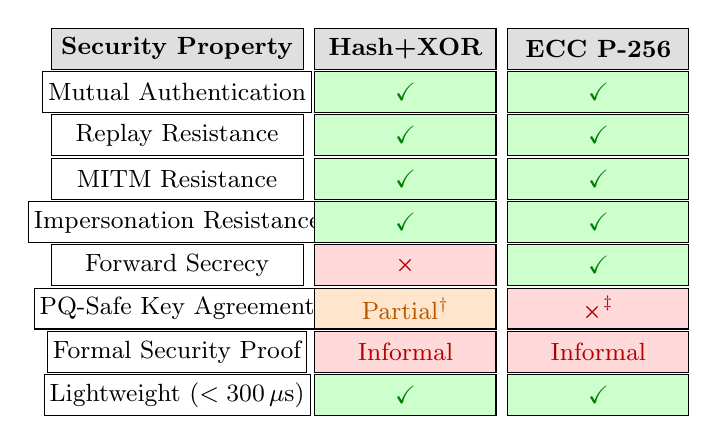
\begin{tikzpicture}[
  font=\small,
  cell/.style={draw, minimum width=2.3cm, minimum height=0.52cm,
               inner sep=2pt, align=center},
  header/.style={cell, fill=gray!25, font=\small\bfseries},
  yes/.style={cell, fill=green!20, text=green!50!black},
  no/.style={cell, fill=red!15, text=red!70!black},
  partial/.style={cell, fill=orange!20, text=orange!70!black},
]
% ---- Header row ----
\node[header, minimum width=3.2cm] (h0) at (0,0) {Security Property};
\node[header] (h1) at (2.9,0) {Hash+XOR};
\node[header] (h2) at (5.35,0) {ECC P-256};

% ---- Row 1: Mutual Authentication ----
\node[cell, minimum width=3.2cm] at (0,-0.55) {Mutual Authentication};
\node[yes]  at (2.9,-0.55) {\checkmark};
\node[yes]  at (5.35,-0.55) {\checkmark};

% ---- Row 2: Replay Resistance ----
\node[cell, minimum width=3.2cm] at (0,-1.1) {Replay Resistance};
\node[yes]  at (2.9,-1.1) {\checkmark};
\node[yes]  at (5.35,-1.1) {\checkmark};

% ---- Row 3: MITM / Tampering Resistance ----
\node[cell, minimum width=3.2cm] at (0,-1.65) {MITM Resistance};
\node[yes]  at (2.9,-1.65) {\checkmark};
\node[yes]  at (5.35,-1.65) {\checkmark};

% ---- Row 4: Impersonation Resistance ----
\node[cell, minimum width=3.2cm] at (0,-2.2) {Impersonation Resistance};
\node[yes]  at (2.9,-2.2) {\checkmark};
\node[yes]  at (5.35,-2.2) {\checkmark};

% ---- Row 5: Forward Secrecy ----
\node[cell, minimum width=3.2cm] at (0,-2.75) {Forward Secrecy};
\node[no]   at (2.9,-2.75) {\texttimes};
\node[yes]  at (5.35,-2.75) {\checkmark};

% ---- Row 6: PQ-Safe Key Agreement ----
\node[cell, minimum width=3.2cm] at (0,-3.3) {PQ-Safe Key Agreement};
\node[partial] at (2.9,-3.3) {Partial$^\dagger$};
\node[no]   at (5.35,-3.3) {\texttimes$^\ddagger$};

% ---- Row 7: Formal Security Proof ----
\node[cell, minimum width=3.2cm] at (0,-3.85) {Formal Security Proof};
\node[no]   at (2.9,-3.85) {Informal};
\node[no]   at (5.35,-3.85) {Informal};

% ---- Row 8: Lightweight (< 300 µs) ----
\node[cell, minimum width=3.2cm] at (0,-4.4) {Lightweight ($<300\,\mu$s)};
\node[yes]  at (2.9,-4.4) {\checkmark};
\node[yes]  at (5.35,-4.4) {\checkmark};

\end{tikzpicture}%
}
\vspace{4pt}

\begin{minipage}{\columnwidth}
\footnotesize
  $^\dagger$ SHA-256 security reduces to $\approx$128-bit equivalent under Grover;
  still considered adequate~\cite{NISTFIPS1804}.\\
  $^\ddagger$ ECDLP is broken in polynomial time by Shor's algorithm~\cite{Shor1997}.
  Forward secrecy holds classically but not against a quantum adversary.
\end{minipage}

\caption{Security property comparison matrix for the Hash+XOR (Ju-Park) and
ECC P-256 schemes. \checkmark = property satisfied; \texttimes = property not
satisfied; Partial = weakened but not broken. Results are based on informal
security analysis (Section~\ref{sec:security}) and primitive-level
post-quantum analysis (Section~\ref{sec:pq}).}
\label{fig:security_matrix}
\end{figure}
% =============================================================================
\begin{figure}[!t]
\centering
\resizebox{\columnwidth}{!}{%
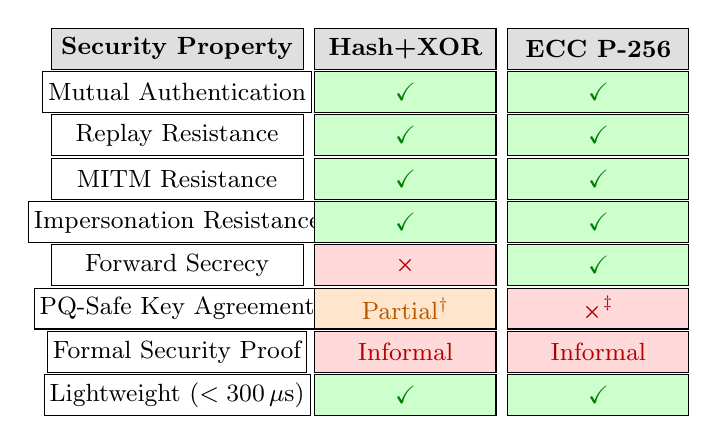
\begin{tikzpicture}[
  font=\small,
  cell/.style={draw, minimum width=2.3cm, minimum height=0.52cm,
               inner sep=2pt, align=center},
  header/.style={cell, fill=gray!25, font=\small\bfseries},
  yes/.style={cell, fill=green!20, text=green!50!black},
  no/.style={cell, fill=red!15, text=red!70!black},
  partial/.style={cell, fill=orange!20, text=orange!70!black},
]
% ---- Header row ----
\node[header, minimum width=3.2cm] (h0) at (0,0) {Security Property};
\node[header] (h1) at (2.9,0) {Hash+XOR};
\node[header] (h2) at (5.35,0) {ECC P-256};

% ---- Row 1: Mutual Authentication ----
\node[cell, minimum width=3.2cm] at (0,-0.55) {Mutual Authentication};
\node[yes]  at (2.9,-0.55) {\checkmark};
\node[yes]  at (5.35,-0.55) {\checkmark};

% ---- Row 2: Replay Resistance ----
\node[cell, minimum width=3.2cm] at (0,-1.1) {Replay Resistance};
\node[yes]  at (2.9,-1.1) {\checkmark};
\node[yes]  at (5.35,-1.1) {\checkmark};

% ---- Row 3: MITM / Tampering Resistance ----
\node[cell, minimum width=3.2cm] at (0,-1.65) {MITM Resistance};
\node[yes]  at (2.9,-1.65) {\checkmark};
\node[yes]  at (5.35,-1.65) {\checkmark};

% ---- Row 4: Impersonation Resistance ----
\node[cell, minimum width=3.2cm] at (0,-2.2) {Impersonation Resistance};
\node[yes]  at (2.9,-2.2) {\checkmark};
\node[yes]  at (5.35,-2.2) {\checkmark};

% ---- Row 5: Forward Secrecy ----
\node[cell, minimum width=3.2cm] at (0,-2.75) {Forward Secrecy};
\node[no]   at (2.9,-2.75) {\texttimes};
\node[yes]  at (5.35,-2.75) {\checkmark};

% ---- Row 6: PQ-Safe Key Agreement ----
\node[cell, minimum width=3.2cm] at (0,-3.3) {PQ-Safe Key Agreement};
\node[partial] at (2.9,-3.3) {Partial$^\dagger$};
\node[no]   at (5.35,-3.3) {\texttimes$^\ddagger$};

% ---- Row 7: Formal Security Proof ----
\node[cell, minimum width=3.2cm] at (0,-3.85) {Formal Security Proof};
\node[no]   at (2.9,-3.85) {Informal};
\node[no]   at (5.35,-3.85) {Informal};

% ---- Row 8: Lightweight (< 300 µs) ----
\node[cell, minimum width=3.2cm] at (0,-4.4) {Lightweight ($<300\,\mu$s)};
\node[yes]  at (2.9,-4.4) {\checkmark};
\node[yes]  at (5.35,-4.4) {\checkmark};

\end{tikzpicture}%
}
\vspace{4pt}

\begin{minipage}{\columnwidth}
\footnotesize
  $^\dagger$ SHA-256 security reduces to $\approx$128-bit equivalent under Grover;
  still considered adequate~\cite{NISTFIPS1804}.\\
  $^\ddagger$ ECDLP is broken in polynomial time by Shor's algorithm~\cite{Shor1997}.
  Forward secrecy holds classically but not against a quantum adversary.
\end{minipage}

\caption{Security property comparison matrix for the Hash+XOR (Ju-Park) and
ECC P-256 schemes. \checkmark = property satisfied; \texttimes = property not
satisfied; Partial = weakened but not broken. Results are based on informal
security analysis (Section~\ref{sec:security}) and primitive-level
post-quantum analysis (Section~\ref{sec:pq}).}
\label{fig:security_matrix}
\end{figure}

The key differentiator is \emph{forward secrecy}: the hash+XOR scheme, as
modelled, derives $\SK$ deterministically from long-term secret material
($\PW_U$), so compromise of $\PW_U$ exposes all past session keys derived
from it. The ECC scheme's use of ephemeral keys prevents this.

\begin{table}[!t]
\caption{Informal Attack Test Results}
\label{tab:attacks}
\centering
\small
\resizebox{0.75\columnwidth}{!}{%
\begin{tabular}{lcc}
\toprule
\textbf{Attack} & \textbf{Hash+XOR} & \textbf{ECC P-256} \\
\midrule
A1 -- Replay            & Pass & Pass \\
A2 -- Delayed Replay    & Pass & Pass \\
A3 -- MITM / Tampering  & Pass & Pass \\
A4 -- Impersonation     & Pass & Pass \\
\bottomrule
\multicolumn{3}{l}{\footnotesize Results from Python test suite;
not a formal proof.}
\end{tabular}%
}
\end{table}

% =============================================================================
\section{Post-Quantum Analysis}
\label{sec:pq}

\subsection{Scope Statement}

This analysis evaluates the quantum resistance of the \emph{cryptographic
primitives} used in each protocol. It does not constitute a security proof
for the complete protocol under a quantum adversary model, and it does not
model adversarial access to quantum oracles in the protocol execution itself.
A full quantum-security analysis would require adaptation of the Dolev-Yao
model to the quantum-accessible random-oracle setting, which is beyond the
scope of this work.

\subsection{Shor's Algorithm and ECDLP}

Shor's algorithm~\cite{Shor1997} solves the integer factorisation and
discrete-logarithm problems in polynomial time on a quantum computer. For
ECC, this means that a sufficiently large quantum computer can recover the
private key $d_S$ from the public key $Q_S = d_S \cdot G$, completely
breaking the key-agreement and authentication mechanisms of the ECC
counterpart. The hash+XOR scheme contains no public-key component, so Shor's
algorithm does not apply to it directly.

\subsection{Grover's Algorithm and SHA-256}

Grover's algorithm~\cite{Grover1996} provides a $\sqrt{N}$ speedup over
classical brute-force search on $N$ inputs. Applied to SHA-256 preimage
search, this reduces the effective security from 256 bits to approximately
128 bits. At 128-bit security, SHA-256 remains practically infeasible for
near-term quantum adversaries and continues to meet NIST security level 1
requirements~\cite{NISTFIPS1804}. XOR masking used in the hash+XOR protocol
inherits this security level because its secrecy depends entirely on the
SHA-256 output used as the mask.

\subsection{Security Margin Table}

Table~\ref{tab:pq_margins} quantifies the quantum security margins.

\begin{table}[!t]
\caption{Post-Quantum Security Margins by Primitive}
\label{tab:pq_margins}
\centering
\small
\resizebox{\columnwidth}{!}{%
\begin{tabular}{lccl}
\toprule
\textbf{Primitive} & \textbf{Classical} & \textbf{Quantum} & \textbf{PQ-Safe?} \\
\midrule
SHA-256 (hash)   & 256 bits & $\approx$128 bits & Yes (Grover only) \\
XOR (w/ SHA-256) & 256 bits & $\approx$128 bits & Yes (inherits above) \\
ECDLP (P-256)    & 128 bits & 0 bits            & \textbf{No} (Shor) \\
\midrule
\textbf{Hash+XOR (overall)}  & 256 bits & $\approx$128 bits & \emph{Partial} \\
\textbf{ECC P-256 (overall)} & 128 bits & 0 bits            & \textbf{No} \\
\bottomrule
\multicolumn{4}{l}{\footnotesize Primitive-level analysis only; does not imply
full-protocol security.}
\end{tabular}%
}
\end{table}

\subsection{Forward Secrecy Under Quantum Threat}

Classically, ECC's forward secrecy provides meaningful protection: past
session keys are secure even if long-term keys are later compromised.
Under a quantum threat, however, Shor's algorithm enables an adversary who
records ciphertext traffic to recover the ephemeral private keys $e_U$ and
$e_S$ from the transmitted public keys $P_U$ and $P_S$, and then compute $Z$
and $\SK$. Consequently, \emph{the forward-secrecy guarantee of ECDH does not
extend to a quantum-capable adversary}. Replacing ECDH with ML-KEM
(NIST FIPS~203~\cite{NISTFIPS203}) would restore quantum-safe forward secrecy.

\subsection{Migration Recommendations}

For cloud-IoT deployments concerned with long-term PQ security, we recommend:
\begin{enumerate}
  \item Replace ECDH key agreement with ML-KEM~768 (NIST FIPS~203) for
    PQ-safe forward secrecy.
  \item Replace ECDSA signatures with ML-DSA (NIST FIPS~204~\cite{NISTFIPS204})
    for quantum-safe entity authentication.
  \item Retain SHA-256 (HMAC mode) for message authentication, noting its
    128-bit PQ security level is adequate under current threat models.
\end{enumerate}

% =============================================================================
\section{Performance Evaluation}
\label{sec:perf}

\subsection{Experimental Setup}

All measurements were taken on a single machine with the following
configuration:
\begin{itemize}
  \item \textbf{CPU:} AMD64 Family~23 Model~96 Stepping~1 (AuthenticAMD)
  \item \textbf{OS:} Windows~11 (64-bit)
  \item \textbf{Runtime:} Python~3.12.6 (CPython, MSC v.1940)
  \item \textbf{Libraries:} \texttt{cryptography}~50.0.1 (OpenSSL backend),
    \texttt{hashlib} (stdlib)
  \item \textbf{Methodology:} 100 protocol executions following 10 warmup
    iterations; wall-clock time measured with \texttt{time.perf\_counter()};
    mean, median, min, max, and standard deviation reported.
\end{itemize}

\begin{quote}
\textbf{Important caveat.} Absolute timing values are dominated by Python
interpreter overhead (function calls, object allocation, dictionary lookups)
and are not directly comparable to native C or embedded-platform benchmarks.
The meaningful metric is the \emph{ratio} between the two protocols measured
under identical conditions.
\end{quote}

\subsection{Computation Time Results}

Table~\ref{tab:timings} reports the measured timings for each protocol phase.

\begin{table}[!t]
\caption{Computation Time ($\mu$s, 100 iterations, 10 warmup)}
\label{tab:timings}
\centering
\small
\resizebox{\columnwidth}{!}{%
\begin{tabular}{lrrr}
\toprule
\textbf{Phase} & \textbf{Hash+XOR} & \textbf{ECC P-256} & \textbf{Ratio} \\
\midrule
Registration (mean) & 31.1\,$\mu$s & 8.7\,$\mu$s  & $3.6\times$ \\
Authentication (mean) & 219.2\,$\mu$s & 262.2\,$\mu$s & $0.84\times$ \\
\midrule
\textbf{Total (mean)}   & \textbf{250.3\,$\mu$s} & \textbf{270.9\,$\mu$s} & $\mathbf{1.08\times}$ \\
Total (median)          & 248.0\,$\mu$s & 264.7\,$\mu$s & $1.06\times$ \\
Total (min)             & 245.8\,$\mu$s & 261.3\,$\mu$s & — \\
Total (max)             & 300.7\,$\mu$s & 416.1\,$\mu$s & — \\
Total (std dev)         & 8.5\,$\mu$s   & 21.2\,$\mu$s  & — \\
\bottomrule
\multicolumn{4}{l}{\footnotesize Source: \texttt{benchmark\_baseline.json}.
Values in $\mu$s (JSON ms $\times$ 1000).}
\end{tabular}%
}
\end{table}

At the total-protocol level, the two implementations are remarkably close:
Hash+XOR completes in 250.3\,$\mu$s on average versus 271.0\,$\mu$s for
ECC---only a 1.08$\times$ difference. This near-parity is a Python-specific
observation: the hash operations (fast C extension via \texttt{hashlib}) and
the ECC operations (fast OpenSSL backend via the \texttt{cryptography} library)
are both highly optimised at the C level, leaving Python's per-call overhead
as the dominant cost for both.

The higher standard deviation for ECC (21.2\,$\mu$s vs.\ 8.5\,$\mu$s) likely
reflects the variable cost of point multiplication, which can exhibit
data-dependent timing behaviour.

\subsection{Communication Overhead}

Table~\ref{tab:comm} reports the communication size breakdown.

\begin{table}[!t]
\caption{Communication Overhead (bits per session)}
\label{tab:comm}
\centering
\small
\resizebox{\columnwidth}{!}{%
\begin{tabular}{lrr}
\toprule
\textbf{Message} & \textbf{Hash+XOR} & \textbf{ECC P-256} \\
\midrule
$M_1$ (User $\to$ CS)  & 1,056 bits & 936 bits \\
$M_2$ (CS $\to$ User)  & 544 bits   & 936 bits \\
Registration            & 2,624 bits & 0 bits$^\dagger$ \\
\midrule
\textbf{Authentication total} & \textbf{1,600 bits} & \textbf{1,872 bits} \\
\textbf{Full total (incl.\ reg.)} & 4,224 bits & 1,872 bits \\
\bottomrule
\multicolumn{3}{l}{\footnotesize $^\dagger$ ECC registration exchanges public
keys (out of band in this skeleton).} \\
\multicolumn{3}{p{\columnwidth}}{\footnotesize
\textbf{Scope note}: The Ju-Park base paper~\cite{JuPark2023} reports
3,776 bits for the full three-party protocol. Our 4,224-bit figure uses
256-bit nonces throughout and covers the U--CS leg only.
No direct comparison is made.}
\end{tabular}%
}
\end{table}

For the authentication-only exchange, ECC is slightly larger (1,872 bits
vs.\ 1,600 bits) because a 520-bit uncompressed P-256 point must be
transmitted. When registration overhead is included, hash+XOR totals 4,224
bits versus 1,872 bits for ECC (a 2.3$\times$ advantage for ECC), because
the hash+XOR registration transmits large credential material.

\subsection{Performance Figure}

Fig.~\ref{fig:performance} presents the data of Tables~\ref{tab:timings}
and~\ref{tab:comm} as grouped bar charts for visual comparison.

% =============================================================================
% fig_performance.tex  —  pgfplots bar chart for performance comparison
% Data source: benchmark_baseline.json (100 iterations, 10 warmup)
%              AMD64 Family 23 Model 96, Windows 11, Python 3.12.6
% Scaled with \resizebox to strictly fit within text width without overflow.
% Include with:  % =============================================================================
% fig_performance.tex  —  pgfplots bar chart for performance comparison
% Data source: benchmark_baseline.json (100 iterations, 10 warmup)
%              AMD64 Family 23 Model 96, Windows 11, Python 3.12.6
% Scaled with \resizebox to strictly fit within text width without overflow.
% Include with:  % =============================================================================
% fig_performance.tex  —  pgfplots bar chart for performance comparison
% Data source: benchmark_baseline.json (100 iterations, 10 warmup)
%              AMD64 Family 23 Model 96, Windows 11, Python 3.12.6
% Scaled with \resizebox to strictly fit within text width without overflow.
% Include with:  \input{figures/fig_performance}
% =============================================================================
\begin{figure*}[!t]
\centering
\resizebox{0.92\textwidth}{!}{%
\begin{tikzpicture}
\begin{groupplot}[
  group style={
    group size=2 by 1,
    horizontal sep=1.4cm
  },
  width=7.2cm,
  height=5.2cm,
  ybar=4pt,
  bar width=16pt,
  enlarge x limits=0.4,
  legend style={at={(0.5,-0.22)}, anchor=north, legend columns=2,
                font=\small},
  symbolic x coords={Registration, Authentication, Total},
  xtick=data,
  x tick label style={font=\small, rotate=15, anchor=east},
  ymin=0,
  grid=major,
  grid style={dashed, gray!40},
]
% ---- LEFT PLOT: Computation Time ----
\nextgroupplot[
  title={\small (a) Computation Time ($\mu$s)},
  ylabel={\small Time ($\mu$s)},
  ytick={0,50,100,150,200,250,300},
  nodes near coords,
  nodes near coords style={font=\tiny, rotate=90, anchor=west},
  every node near coord/.append style={xshift=2pt, yshift=2pt},
]
% Ju-Park (Hash+XOR) — values in µs from JSON (ms × 1000)
\addplot[fill=blue!60, draw=blue!80] coordinates {
  (Registration,  31.1)
  (Authentication, 219.2)
  (Total,          250.3)
};
\addlegendentry{Hash+XOR (Ju-Park)}

% ECC P-256 — values in µs from JSON
\addplot[fill=red!60, draw=red!80] coordinates {
  (Registration,   8.7)
  (Authentication, 262.2)
  (Total,          270.9)
};
\addlegendentry{ECC P-256}

% ---- RIGHT PLOT: Communication Overhead ----
\nextgroupplot[
  title={\small (b) Communication Overhead (bits)},
  ylabel={\small Message Size (bits)},
  symbolic x coords={Total},
  xtick=data,
  ytick={0,500,1000,1500,2000,2500,3000,3500,4000,4500},
  ymax=4800,
  nodes near coords,
  nodes near coords style={font=\small},
]
\addplot[fill=blue!60, draw=blue!80] coordinates {
  (Total, 4224)
};

\addplot[fill=red!60, draw=red!80] coordinates {
  (Total, 1872)
};
\end{groupplot}
\end{tikzpicture}%
}
\caption{Performance comparison between the Hash+XOR scheme (Ju-Park) and
the ECC P-256 counterpart. (a)~Computation times measured over 100 iterations
(10 warmup) on an AMD Athlon/Ryzen class CPU (AMD64 Family~23 Model~96),
Windows~11, Python~3.12.6. Values reflect Python interpreter overhead and
are not directly comparable to native-C benchmarks. Ratios are the
meaningful metric. (b)~Communication overhead in bits per complete
authentication session. ECC achieves~$\approx 2.3\times$ lower overhead
due to compact ephemeral public keys and nonces, despite carrying 520-bit
uncompressed P-256 points.}
\label{fig:performance}
\end{figure*}

% =============================================================================
\begin{figure*}[!t]
\centering
\resizebox{0.92\textwidth}{!}{%
\begin{tikzpicture}
\begin{groupplot}[
  group style={
    group size=2 by 1,
    horizontal sep=1.4cm
  },
  width=7.2cm,
  height=5.2cm,
  ybar=4pt,
  bar width=16pt,
  enlarge x limits=0.4,
  legend style={at={(0.5,-0.22)}, anchor=north, legend columns=2,
                font=\small},
  symbolic x coords={Registration, Authentication, Total},
  xtick=data,
  x tick label style={font=\small, rotate=15, anchor=east},
  ymin=0,
  grid=major,
  grid style={dashed, gray!40},
]
% ---- LEFT PLOT: Computation Time ----
\nextgroupplot[
  title={\small (a) Computation Time ($\mu$s)},
  ylabel={\small Time ($\mu$s)},
  ytick={0,50,100,150,200,250,300},
  nodes near coords,
  nodes near coords style={font=\tiny, rotate=90, anchor=west},
  every node near coord/.append style={xshift=2pt, yshift=2pt},
]
% Ju-Park (Hash+XOR) — values in µs from JSON (ms × 1000)
\addplot[fill=blue!60, draw=blue!80] coordinates {
  (Registration,  31.1)
  (Authentication, 219.2)
  (Total,          250.3)
};
\addlegendentry{Hash+XOR (Ju-Park)}

% ECC P-256 — values in µs from JSON
\addplot[fill=red!60, draw=red!80] coordinates {
  (Registration,   8.7)
  (Authentication, 262.2)
  (Total,          270.9)
};
\addlegendentry{ECC P-256}

% ---- RIGHT PLOT: Communication Overhead ----
\nextgroupplot[
  title={\small (b) Communication Overhead (bits)},
  ylabel={\small Message Size (bits)},
  symbolic x coords={Total},
  xtick=data,
  ytick={0,500,1000,1500,2000,2500,3000,3500,4000,4500},
  ymax=4800,
  nodes near coords,
  nodes near coords style={font=\small},
]
\addplot[fill=blue!60, draw=blue!80] coordinates {
  (Total, 4224)
};

\addplot[fill=red!60, draw=red!80] coordinates {
  (Total, 1872)
};
\end{groupplot}
\end{tikzpicture}%
}
\caption{Performance comparison between the Hash+XOR scheme (Ju-Park) and
the ECC P-256 counterpart. (a)~Computation times measured over 100 iterations
(10 warmup) on an AMD Athlon/Ryzen class CPU (AMD64 Family~23 Model~96),
Windows~11, Python~3.12.6. Values reflect Python interpreter overhead and
are not directly comparable to native-C benchmarks. Ratios are the
meaningful metric. (b)~Communication overhead in bits per complete
authentication session. ECC achieves~$\approx 2.3\times$ lower overhead
due to compact ephemeral public keys and nonces, despite carrying 520-bit
uncompressed P-256 points.}
\label{fig:performance}
\end{figure*}

% =============================================================================
\begin{figure*}[!t]
\centering
\resizebox{0.92\textwidth}{!}{%
\begin{tikzpicture}
\begin{groupplot}[
  group style={
    group size=2 by 1,
    horizontal sep=1.4cm
  },
  width=7.2cm,
  height=5.2cm,
  ybar=4pt,
  bar width=16pt,
  enlarge x limits=0.4,
  legend style={at={(0.5,-0.22)}, anchor=north, legend columns=2,
                font=\small},
  symbolic x coords={Registration, Authentication, Total},
  xtick=data,
  x tick label style={font=\small, rotate=15, anchor=east},
  ymin=0,
  grid=major,
  grid style={dashed, gray!40},
]
% ---- LEFT PLOT: Computation Time ----
\nextgroupplot[
  title={\small (a) Computation Time ($\mu$s)},
  ylabel={\small Time ($\mu$s)},
  ytick={0,50,100,150,200,250,300},
  nodes near coords,
  nodes near coords style={font=\tiny, rotate=90, anchor=west},
  every node near coord/.append style={xshift=2pt, yshift=2pt},
]
% Ju-Park (Hash+XOR) — values in µs from JSON (ms × 1000)
\addplot[fill=blue!60, draw=blue!80] coordinates {
  (Registration,  31.1)
  (Authentication, 219.2)
  (Total,          250.3)
};
\addlegendentry{Hash+XOR (Ju-Park)}

% ECC P-256 — values in µs from JSON
\addplot[fill=red!60, draw=red!80] coordinates {
  (Registration,   8.7)
  (Authentication, 262.2)
  (Total,          270.9)
};
\addlegendentry{ECC P-256}

% ---- RIGHT PLOT: Communication Overhead ----
\nextgroupplot[
  title={\small (b) Communication Overhead (bits)},
  ylabel={\small Message Size (bits)},
  symbolic x coords={Total},
  xtick=data,
  ytick={0,500,1000,1500,2000,2500,3000,3500,4000,4500},
  ymax=4800,
  nodes near coords,
  nodes near coords style={font=\small},
]
\addplot[fill=blue!60, draw=blue!80] coordinates {
  (Total, 4224)
};

\addplot[fill=red!60, draw=red!80] coordinates {
  (Total, 1872)
};
\end{groupplot}
\end{tikzpicture}%
}
\caption{Performance comparison between the Hash+XOR scheme (Ju-Park) and
the ECC P-256 counterpart. (a)~Computation times measured over 100 iterations
(10 warmup) on an AMD Athlon/Ryzen class CPU (AMD64 Family~23 Model~96),
Windows~11, Python~3.12.6. Values reflect Python interpreter overhead and
are not directly comparable to native-C benchmarks. Ratios are the
meaningful metric. (b)~Communication overhead in bits per complete
authentication session. ECC achieves~$\approx 2.3\times$ lower overhead
due to compact ephemeral public keys and nonces, despite carrying 520-bit
uncompressed P-256 points.}
\label{fig:performance}
\end{figure*}


\subsection{Throughput}

At 250.3\,$\mu$s per round, the hash+XOR scheme achieves approximately
3,995 authentications per second; ECC achieves approximately 3,692 per
second. Both are high enough for typical cloud-IoT scenarios where
authentication events occur on the order of seconds to minutes.

% =============================================================================
\section{Additional Features}
\label{sec:additional}

\subsection{Reduced Round-Trip Variant}

In addition to the primary Ju-Park skeleton and ECC counterpart, a
\emph{reduced round-trip} variant was implemented that consolidates the
login and verification steps into a single message exchange, reducing the
protocol from four messages to three. Benchmarks (from
\texttt{benchmark\_baseline.json}) show a total authentication mean of
222.3\,$\mu$s (median 218.6\,$\mu$s, std dev 11.7\,$\mu$s), representing an
approximately 12\% latency reduction versus the full Ju-Park skeleton. This
comes at the cost of omitting the server's explicit key-confirmation step,
which weakens the mutual-authentication guarantee.

\subsection{ML-KEM-768 Prototype}

A proof-of-concept ML-KEM-768 integration (NIST FIPS~203~\cite{NISTFIPS203})
was prototyped in the codebase to demonstrate the migration path described in
Section~\ref{sec:pq}. ML-KEM replaces the ECDH key-agreement primitive with a
module-lattice-based key-encapsulation mechanism, providing quantum-safe
forward secrecy without relying on ECDLP hardness. Full benchmarking and
protocol integration of the ML-KEM variant is left as future work.

% =============================================================================
\section{Limitations}
\label{sec:limitations}

The following limitations should be considered when interpreting the results
of this study:

\begin{enumerate}
  \item \textbf{Skeleton scope.} The hash+XOR implementation covers the
    User--Cloud Server leg only and omits the Control-Server forwarding and
    key-confirmation steps. The resulting 4,224-bit communication figure is
    not comparable to the Ju-Park paper's 3,776-bit figure~\cite{JuPark2023}.

  \item \textbf{Informal security analysis.} All security evaluation is based
    on Python test cases. No formal tool (ProVerif, Tamarin, etc.) was applied
    in this work; test results demonstrate resistance under the implemented
    logic but do not constitute cryptographic proofs.

  \item \textbf{Python performance overhead.} Measured timings include
    substantial Python interpreter overhead. Absolute values would differ
    significantly on embedded C/Rust implementations. Ratios between the two
    schemes are the reliable comparison metric.

  \item \textbf{Primitive-level PQ analysis.} The post-quantum analysis in
    Section~\ref{sec:pq} concerns individual cryptographic primitives. A
    full-protocol PQ security argument (e.g., in the quantum-accessible
    random-oracle model) is outside the scope of this work.

  \item \textbf{No forward secrecy in hash+XOR.} As modelled, the hash+XOR
    scheme derives session keys deterministically from the long-term password.
    This is a known structural limitation, not a flaw introduced by our
    implementation.

  \item \textbf{Single-platform benchmark.} All experiments were conducted on
    one machine running Windows~11. Cross-platform or embedded-hardware
    validation has not been performed.
\end{enumerate}

% =============================================================================
\section{Conclusion and Future Work}
\label{sec:conclusion}

This paper presented a direct implementation and comparison of a lightweight
hash+XOR mutual authentication scheme (adapted from Ju-Park 2023) and an
ECC P-256 counterpart, evaluated for both practical performance and
post-quantum readiness.

The key findings are:
\begin{itemize}
  \item Under Python, the two protocols exhibit near-equal total latency
    (250\,$\mu$s vs.\ 271\,$\mu$s, a 1.08$\times$ ratio), with ECC achieving
    2.3$\times$ lower full-session communication overhead when registration is
    excluded, but 2.3$\times$ higher overhead when included (due to XOR
    registration credential size).
  \item The hash+XOR scheme's SHA-256 primitive retains $\approx$128-bit
    security under Grover's algorithm and is thus partially quantum-resilient,
    but the scheme lacks forward secrecy.
  \item The ECC counterpart provides forward secrecy classically but ECDLP is
    solvable in polynomial quantum time by Shor's algorithm, offering no
    PQ-safe key-agreement primitive.
  \item Neither scheme is fully post-quantum secure; migration to ML-KEM
    (FIPS~203) for key agreement and ML-DSA (FIPS~204) for authentication is
    the recommended path.
\end{itemize}

\textbf{Future work} includes: (1) full three-party Control-Server leg
implementation; (2) formal verification using ProVerif or Tamarin; (3) ML-KEM
integration and benchmarking; (4) embedded-hardware (ARM Cortex-M) performance
evaluation; (5) extension of the PQ analysis to the full protocol in the
quantum-accessible random-oracle model.

% =============================================================================
\section*{Data and Code Availability}

The dataset used in this study is a synthetic IoT authentication benchmark
generated programmatically using Python. No real user or device data was
collected. The benchmark data are available as
\texttt{research/results/benchmark\_baseline.json} in the project repository.

The complete source code---including protocol implementations, test harness,
and benchmark scripts---is available at the project repository. Reproduction
instructions are provided in \texttt{REPRODUCE.md}.

% =============================================================================
\section*{Author Contributions}

S.~P.~S.~Raikuni conceived the study design, implemented all protocol code,
conducted the benchmarks and security tests, performed the post-quantum
analysis, and wrote the manuscript. Dr.~Karthika~V provided academic
supervision and guidance on the research direction.

% =============================================================================
\section*{Acknowledgment}

The author thanks Dr.~Karthika~V (VIT Chennai) for her guidance and support
throughout this research. The author also acknowledges the open-source
developers of the \texttt{cryptography} Python library and the maintainers of
IEEEtran for providing the typesetting infrastructure used in this work.

% =============================================================================
\bibliographystyle{IEEEtran}
\bibliography{references}

\end{document}
